\documentclass[twoside]{book}

% Packages required by doxygen
\usepackage{fixltx2e}
\usepackage{calc}
\usepackage{doxygen}
\usepackage[export]{adjustbox} % also loads graphicx
\usepackage{graphicx}
\usepackage[utf8]{inputenc}
\usepackage{makeidx}
\usepackage{multicol}
\usepackage{multirow}
\PassOptionsToPackage{warn}{textcomp}
\usepackage{textcomp}
\usepackage[nointegrals]{wasysym}
\usepackage[table]{xcolor}

% Font selection
\usepackage[T1]{fontenc}
\usepackage[scaled=.90]{helvet}
\usepackage{courier}
\usepackage{amssymb}
\usepackage{sectsty}
\renewcommand{\familydefault}{\sfdefault}
\allsectionsfont{%
  \fontseries{bc}\selectfont%
  \color{darkgray}%
}
\renewcommand{\DoxyLabelFont}{%
  \fontseries{bc}\selectfont%
  \color{darkgray}%
}
\newcommand{\+}{\discretionary{\mbox{\scriptsize$\hookleftarrow$}}{}{}}

% Page & text layout
\usepackage{geometry}
\geometry{%
  a4paper,%
  top=2.5cm,%
  bottom=2.5cm,%
  left=2.5cm,%
  right=2.5cm%
}
\tolerance=750
\hfuzz=15pt
\hbadness=750
\setlength{\emergencystretch}{15pt}
\setlength{\parindent}{0cm}
\setlength{\parskip}{3ex plus 2ex minus 2ex}
\makeatletter
\renewcommand{\paragraph}{%
  \@startsection{paragraph}{4}{0ex}{-1.0ex}{1.0ex}{%
    \normalfont\normalsize\bfseries\SS@parafont%
  }%
}
\renewcommand{\subparagraph}{%
  \@startsection{subparagraph}{5}{0ex}{-1.0ex}{1.0ex}{%
    \normalfont\normalsize\bfseries\SS@subparafont%
  }%
}
\makeatother

% Headers & footers
\usepackage{fancyhdr}
\pagestyle{fancyplain}
\fancyhead[LE]{\fancyplain{}{\bfseries\thepage}}
\fancyhead[CE]{\fancyplain{}{}}
\fancyhead[RE]{\fancyplain{}{\bfseries\leftmark}}
\fancyhead[LO]{\fancyplain{}{\bfseries\rightmark}}
\fancyhead[CO]{\fancyplain{}{}}
\fancyhead[RO]{\fancyplain{}{\bfseries\thepage}}
\fancyfoot[LE]{\fancyplain{}{}}
\fancyfoot[CE]{\fancyplain{}{}}
\fancyfoot[RE]{\fancyplain{}{\bfseries\scriptsize Generated by Doxygen }}
\fancyfoot[LO]{\fancyplain{}{\bfseries\scriptsize Generated by Doxygen }}
\fancyfoot[CO]{\fancyplain{}{}}
\fancyfoot[RO]{\fancyplain{}{}}
\renewcommand{\footrulewidth}{0.4pt}
\renewcommand{\chaptermark}[1]{%
  \markboth{#1}{}%
}
\renewcommand{\sectionmark}[1]{%
  \markright{\thesection\ #1}%
}

% Indices & bibliography
\usepackage{natbib}
\usepackage[titles]{tocloft}
\setcounter{tocdepth}{3}
\setcounter{secnumdepth}{5}
\makeindex

% Hyperlinks (required, but should be loaded last)
\usepackage{ifpdf}
\ifpdf
  \usepackage[pdftex,pagebackref=true]{hyperref}
\else
  \usepackage[ps2pdf,pagebackref=true]{hyperref}
\fi
\hypersetup{%
  colorlinks=true,%
  linkcolor=blue,%
  citecolor=blue,%
  unicode%
}

% Custom commands
\newcommand{\clearemptydoublepage}{%
  \newpage{\pagestyle{empty}\cleardoublepage}%
}

\usepackage{caption}
\captionsetup{labelsep=space,justification=centering,font={bf},singlelinecheck=off,skip=4pt,position=top}

%===== C O N T E N T S =====

\begin{document}

% Titlepage & ToC
\hypersetup{pageanchor=false,
             bookmarksnumbered=true,
             pdfencoding=unicode
            }
\pagenumbering{alph}
\begin{titlepage}
\vspace*{7cm}
\begin{center}%
{\Large Bellerophon }\\
\vspace*{1cm}
{\large Generated by Doxygen 1.8.12}\\
\end{center}
\end{titlepage}
\clearemptydoublepage
\pagenumbering{roman}
\tableofcontents
\clearemptydoublepage
\pagenumbering{arabic}
\hypersetup{pageanchor=true}

%--- Begin generated contents ---
\chapter{Module Index}
\section{Modules}
Here is a list of all modules\+:\begin{DoxyCompactList}
\item \contentsline{section}{F\+AP Floating Point Shifting functions}{\pageref{group__FAP__FP__SHIFTING__FUNCTIONS}}{}
\item \contentsline{section}{Input/\+Output overloaded operators}{\pageref{group__OPERATOR__OVERLOAD__INPUT__OUTPUT}}{}
\end{DoxyCompactList}

\chapter{Namespace Index}
\section{Namespace List}
Here is a list of all documented namespaces with brief descriptions\+:\begin{DoxyCompactList}
\item\contentsline{section}{\hyperlink{namespacebellerophon_1_1fs}{bellerophon\+::fs} \\*Filesystem functions }{\pageref{namespacebellerophon_1_1fs}}{}
\item\contentsline{section}{\hyperlink{namespacebellerophon_1_1syntax}{bellerophon\+::syntax} \\*Syntax checker }{\pageref{namespacebellerophon_1_1syntax}}{}
\end{DoxyCompactList}

\chapter{Hierarchical Index}
\section{Class Hierarchy}
This inheritance list is sorted roughly, but not completely, alphabetically\+:\begin{DoxyCompactList}
\item \contentsline{section}{bellerophon\+:\+:core\+:\+:Aprx\+Context}{\pageref{classbellerophon_1_1core_1_1AprxContext}}{}
\begin{DoxyCompactList}
\item \contentsline{section}{bellerophon\+:\+:flap\+Context\+:\+:Flap\+Aprx\+Context}{\pageref{classbellerophon_1_1flapContext_1_1FlapAprxContext}}{}
\end{DoxyCompactList}
\item Aprx\+Context\begin{DoxyCompactList}
\item \contentsline{section}{Loop\+Perforation\+Context}{\pageref{classLoopPerforationContext}}{}
\end{DoxyCompactList}
\item \contentsline{section}{bellerophon\+:\+:core\+:\+:Aprx\+Location}{\pageref{structbellerophon_1_1core_1_1AprxLocation}}{}
\item \contentsline{section}{bellerophon\+:\+:core\+:\+:Aprx\+Technique}{\pageref{classbellerophon_1_1core_1_1AprxTechnique}}{}
\begin{DoxyCompactList}
\item \contentsline{section}{Flap\+Aprx\+Technique}{\pageref{classFlapAprxTechnique}}{}
\end{DoxyCompactList}
\item \contentsline{section}{bellerophon\+:\+:log\+:\+:Bellerophon\+Logger}{\pageref{classbellerophon_1_1log_1_1BellerophonLogger}}{}
\item \contentsline{section}{bellerophon\+:\+:tool\+:\+:Bellerophon\+Tool}{\pageref{classbellerophon_1_1tool_1_1BellerophonTool}}{}
\item \contentsline{section}{bellerophon\+:\+:core\+:\+:Evolution\+Context}{\pageref{classbellerophon_1_1core_1_1EvolutionContext}}{}
\item \contentsline{section}{bellerophon\+:\+:engine\+:\+:Execution\+Engine\+Helper}{\pageref{classbellerophon_1_1engine_1_1ExecutionEngineHelper}}{}
\item \contentsline{section}{fap\+:\+:Floating\+Point\+Type}{\pageref{classfap_1_1FloatingPointType}}{}
\item \contentsline{section}{fap\+:\+:Float\+Prec\+Ty}{\pageref{structfap_1_1FloatPrecTy}}{}
\item \contentsline{section}{fap\+:\+:Integer\+Type}{\pageref{classfap_1_1IntegerType}}{}
\item \contentsline{section}{bellerophon\+:\+:engine\+:\+:Module\+Helper}{\pageref{classbellerophon_1_1engine_1_1ModuleHelper}}{}
\item moeo\+Eval\+Func\begin{DoxyCompactList}
\item \contentsline{section}{bellerophon\+:\+:core\+:\+:aprx\+Eval}{\pageref{classbellerophon_1_1core_1_1aprxEval}}{}
\end{DoxyCompactList}
\item moeo\+Objective\+Vector\+Traits\begin{DoxyCompactList}
\item \contentsline{section}{bellerophon\+:\+:core\+:\+:Aprx\+Objective\+Vector\+Traits}{\pageref{classbellerophon_1_1core_1_1AprxObjectiveVectorTraits}}{}
\end{DoxyCompactList}
\item moeo\+Real\+Vector\begin{DoxyCompactList}
\item \contentsline{section}{bellerophon\+:\+:core\+:\+:aprx}{\pageref{classbellerophon_1_1core_1_1aprx}}{}
\end{DoxyCompactList}
\end{DoxyCompactList}

\chapter{Class Index}
\section{Class List}
Here are the classes, structs, unions and interfaces with brief descriptions\+:\begin{DoxyCompactList}
\item\contentsline{section}{\hyperlink{classbellerophon_1_1core_1_1aprx}{bellerophon\+::core\+::aprx} }{\pageref{classbellerophon_1_1core_1_1aprx}}{}
\item\contentsline{section}{\hyperlink{classbellerophon_1_1core_1_1AprxContext}{bellerophon\+::core\+::\+Aprx\+Context} }{\pageref{classbellerophon_1_1core_1_1AprxContext}}{}
\item\contentsline{section}{\hyperlink{classbellerophon_1_1core_1_1aprxEval}{bellerophon\+::core\+::aprx\+Eval} }{\pageref{classbellerophon_1_1core_1_1aprxEval}}{}
\item\contentsline{section}{\hyperlink{structbellerophon_1_1core_1_1AprxLocation}{bellerophon\+::core\+::\+Aprx\+Location} \\*Bind between an \hyperlink{classbellerophon_1_1core_1_1AprxTechnique}{Aprx\+Technique} and an aprx\+Grade that can be \textquotesingle{}accumulated\textquotesingle{} }{\pageref{structbellerophon_1_1core_1_1AprxLocation}}{}
\item\contentsline{section}{\hyperlink{classbellerophon_1_1core_1_1AprxObjectiveVectorTraits}{bellerophon\+::core\+::\+Aprx\+Objective\+Vector\+Traits} }{\pageref{classbellerophon_1_1core_1_1AprxObjectiveVectorTraits}}{}
\item\contentsline{section}{\hyperlink{classbellerophon_1_1core_1_1AprxTechnique}{bellerophon\+::core\+::\+Aprx\+Technique} \\*Interface that abstracts an approximation strategy }{\pageref{classbellerophon_1_1core_1_1AprxTechnique}}{}
\item\contentsline{section}{\hyperlink{classbellerophon_1_1log_1_1BellerophonLogger}{bellerophon\+::log\+::\+Bellerophon\+Logger} \\*Bellero\+Logger Class, provides all functions for the logging }{\pageref{classbellerophon_1_1log_1_1BellerophonLogger}}{}
\item\contentsline{section}{\hyperlink{classbellerophon_1_1tool_1_1BellerophonTool}{bellerophon\+::tool\+::\+Bellerophon\+Tool} }{\pageref{classbellerophon_1_1tool_1_1BellerophonTool}}{}
\item\contentsline{section}{\hyperlink{classbellerophon_1_1core_1_1EvolutionContext}{bellerophon\+::core\+::\+Evolution\+Context} }{\pageref{classbellerophon_1_1core_1_1EvolutionContext}}{}
\item\contentsline{section}{\hyperlink{classbellerophon_1_1engine_1_1ExecutionEngineHelper}{bellerophon\+::engine\+::\+Execution\+Engine\+Helper} \\*Helper class to interact with the L\+L\+VM execution engine }{\pageref{classbellerophon_1_1engine_1_1ExecutionEngineHelper}}{}
\item\contentsline{section}{\hyperlink{classbellerophon_1_1flapContext_1_1FlapAprxContext}{bellerophon\+::flap\+Context\+::\+Flap\+Aprx\+Context} }{\pageref{classbellerophon_1_1flapContext_1_1FlapAprxContext}}{}
\item\contentsline{section}{\hyperlink{classFlapAprxTechnique}{Flap\+Aprx\+Technique} }{\pageref{classFlapAprxTechnique}}{}
\item\contentsline{section}{\hyperlink{classfap_1_1FloatingPointType}{fap\+::\+Floating\+Point\+Type} \\*Class for floating point type }{\pageref{classfap_1_1FloatingPointType}}{}
\item\contentsline{section}{\hyperlink{structfap_1_1FloatPrecTy}{fap\+::\+Float\+Prec\+Ty} \\*Precision type }{\pageref{structfap_1_1FloatPrecTy}}{}
\item\contentsline{section}{\hyperlink{classfap_1_1IntegerType}{fap\+::\+Integer\+Type} \\*Class for integer type }{\pageref{classfap_1_1IntegerType}}{}
\item\contentsline{section}{\hyperlink{classLoopPerforationContext}{Loop\+Perforation\+Context} }{\pageref{classLoopPerforationContext}}{}
\item\contentsline{section}{\hyperlink{classbellerophon_1_1engine_1_1ModuleHelper}{bellerophon\+::engine\+::\+Module\+Helper} }{\pageref{classbellerophon_1_1engine_1_1ModuleHelper}}{}
\end{DoxyCompactList}

\chapter{File Index}
\section{File List}
Here is a list of all documented files with brief descriptions\+:\begin{DoxyCompactList}
\item\contentsline{section}{/home/ntonjeta/sharedfolder/bellerophon/include/\hyperlink{Log_8h}{Log.\+h} \\*This file contains a logging facility }{\pageref{Log_8h}}{}
\item\contentsline{section}{/home/ntonjeta/sharedfolder/bellerophon/include/\hyperlink{Utils_8h}{Utils.\+h} \\*This file contains a utility functions }{\pageref{Utils_8h}}{}
\item\contentsline{section}{/home/ntonjeta/sharedfolder/bellerophon/include/\+Core/{\bfseries Aprx\+Context.\+h} }{\pageref{AprxContext_8h}}{}
\item\contentsline{section}{/home/ntonjeta/sharedfolder/bellerophon/include/\+Core/{\bfseries Aprx\+Technique.\+h} }{\pageref{AprxTechnique_8h}}{}
\item\contentsline{section}{/home/ntonjeta/sharedfolder/bellerophon/include/\+Core/{\bfseries Evolution\+Context.\+h} }{\pageref{EvolutionContext_8h}}{}
\item\contentsline{section}{/home/ntonjeta/sharedfolder/bellerophon/include/\+Execution\+Engine\+Helper/{\bfseries Execution\+Engine\+Helper.\+h} }{\pageref{ExecutionEngineHelper_8h}}{}
\item\contentsline{section}{/home/ntonjeta/sharedfolder/bellerophon/include/\+Plugins/\hyperlink{Context_8h}{Context.\+h} \\*This file makes visible Approximate Context }{\pageref{Context_8h}}{}
\item\contentsline{section}{/home/ntonjeta/sharedfolder/bellerophon/include/\+Plugins/{\bfseries Loop\+Perforation\+Aprx.\+h} }{\pageref{LoopPerforationAprx_8h}}{}
\item\contentsline{section}{/home/ntonjeta/sharedfolder/bellerophon/include/\+Plugins/\+F\+L\+A\+P/{\bfseries fap.\+h} }{\pageref{fap_8h}}{}
\item\contentsline{section}{/home/ntonjeta/sharedfolder/bellerophon/include/\+Plugins/\+F\+L\+A\+P/{\bfseries Flap\+Aprx\+Context.\+h} }{\pageref{FlapAprxContext_8h}}{}
\item\contentsline{section}{/home/ntonjeta/sharedfolder/bellerophon/include/\+Plugins/\+F\+L\+A\+P/{\bfseries Flap\+Aprx\+Technique.\+h} }{\pageref{FlapAprxTechnique_8h}}{}
\item\contentsline{section}{/home/ntonjeta/sharedfolder/bellerophon/include/\+Tool/{\bfseries Bellerophon\+Tool.\+h} }{\pageref{BellerophonTool_8h}}{}
\item\contentsline{section}{/home/ntonjeta/sharedfolder/bellerophon/src/\hyperlink{Log_8cpp}{Log.\+cpp} \\*This file contains a logging facility }{\pageref{Log_8cpp}}{}
\item\contentsline{section}{/home/ntonjeta/sharedfolder/bellerophon/src/\hyperlink{Utils_8cpp}{Utils.\+cpp} \\*This file implements a utility functions }{\pageref{Utils_8cpp}}{}
\end{DoxyCompactList}

\chapter{Module Documentation}
\hypertarget{group__FAP__FP__SHIFTING__FUNCTIONS}{}\section{F\+AP Floating Point Shifting functions}
\label{group__FAP__FP__SHIFTING__FUNCTIONS}\index{F\+A\+P Floating Point Shifting functions@{F\+A\+P Floating Point Shifting functions}}
\subsection*{Functions}
\begin{DoxyCompactItemize}
\item 
\hypertarget{group__FAP__FP__SHIFTING__FUNCTIONS_ga0ed6cc29d7fb322732e4def6f3e227ee}{}\label{group__FAP__FP__SHIFTING__FUNCTIONS_ga0ed6cc29d7fb322732e4def6f3e227ee} 
void {\bfseries fap\+\_\+shift\+\_\+right\+\_\+} (uint128\+\_\+t $\ast$, int to\+\_\+shift, uint8\+\_\+t $\ast$grs)
\item 
\hypertarget{group__FAP__FP__SHIFTING__FUNCTIONS_ga5fb1f3adac7181da3245ba307dcd1c93}{}\label{group__FAP__FP__SHIFTING__FUNCTIONS_ga5fb1f3adac7181da3245ba307dcd1c93} 
void {\bfseries fap\+\_\+shift\+\_\+left\+\_\+} (uint128\+\_\+t $\ast$, int to\+\_\+shift, uint8\+\_\+t $\ast$grs)
\end{DoxyCompactItemize}


\subsection{Detailed Description}

\hypertarget{group__OPERATOR__OVERLOAD__INPUT__OUTPUT}{}\section{Input/\+Output overloaded operators}
\label{group__OPERATOR__OVERLOAD__INPUT__OUTPUT}\index{Input/\+Output overloaded operators@{Input/\+Output overloaded operators}}
\subsection*{Functions}
\begin{DoxyCompactItemize}
\item 
\hypertarget{group__OPERATOR__OVERLOAD__INPUT__OUTPUT_ga0d9949e450b50364788252bc970bbaa7}{}\label{group__OPERATOR__OVERLOAD__INPUT__OUTPUT_ga0d9949e450b50364788252bc970bbaa7} 
\+::std\+::ostream \& {\bfseries operator$<$$<$} (\+::std\+::ostream \&, const \+::\hyperlink{classfap_1_1FloatingPointType}{fap\+::\+Floating\+Point\+Type} \&)
\item 
\hypertarget{group__OPERATOR__OVERLOAD__INPUT__OUTPUT_gad02d46ac3ef92ecf0388bce718713bb9}{}\label{group__OPERATOR__OVERLOAD__INPUT__OUTPUT_gad02d46ac3ef92ecf0388bce718713bb9} 
\+::std\+::ostream \& {\bfseries operator$<$$<$} (\+::std\+::ostream \&, const \+::\hyperlink{classfap_1_1IntegerType}{fap\+::\+Integer\+Type} \&)
\end{DoxyCompactItemize}


\subsection{Detailed Description}

\chapter{Namespace Documentation}
\hypertarget{namespacebellerophon_1_1fs}{}\section{bellerophon\+:\+:fs Namespace Reference}
\label{namespacebellerophon_1_1fs}\index{bellerophon\+::fs@{bellerophon\+::fs}}


Filesystem functions.  


\subsection*{Functions}
\begin{DoxyCompactItemize}
\item 
char \hyperlink{namespacebellerophon_1_1fs_a5fdf1fe521ee409381f36acf1457a858}{get\+Path\+Separator} ()
\item 
std\+::string \hyperlink{namespacebellerophon_1_1fs_acd4c35b60168bc21d107608e56128664}{get\+Parent\+Path} (const std\+::string \&)
\begin{DoxyCompactList}\small\item\em Get the parent directory of a path. \end{DoxyCompactList}\item 
bool \hyperlink{namespacebellerophon_1_1fs_a863646cc2d1337eb038f7fdb45012a3a}{create\+Directories} (const llvm\+::\+Twine \&path, bool ignore\+Existing=true)
\begin{DoxyCompactList}\small\item\em Create directories e sub-\/directories. \end{DoxyCompactList}\item 
\hypertarget{namespacebellerophon_1_1fs_ad2da81a3ede3323f05544977de6d3408}{}\label{namespacebellerophon_1_1fs_ad2da81a3ede3323f05544977de6d3408} 
void {\bfseries delete\+Directory} (const llvm\+::\+Twine \&path)
\end{DoxyCompactItemize}
\subsection*{Variables}
\begin{DoxyCompactItemize}
\item 
\hypertarget{namespacebellerophon_1_1fs_a058ef4b019d24eea183b04e5da71c288}{}\label{namespacebellerophon_1_1fs_a058ef4b019d24eea183b04e5da71c288} 
const char {\bfseries path\+Sep}
\end{DoxyCompactItemize}


\subsection{Detailed Description}
Filesystem functions. 

\subsection{Function Documentation}
\hypertarget{namespacebellerophon_1_1fs_a863646cc2d1337eb038f7fdb45012a3a}{}\label{namespacebellerophon_1_1fs_a863646cc2d1337eb038f7fdb45012a3a} 
\index{bellerophon\+::fs@{bellerophon\+::fs}!create\+Directories@{create\+Directories}}
\index{create\+Directories@{create\+Directories}!bellerophon\+::fs@{bellerophon\+::fs}}
\subsubsection{\texorpdfstring{create\+Directories()}{createDirectories()}}
{\footnotesize\ttfamily bool bellerophon\+::fs\+::create\+Directories (\begin{DoxyParamCaption}\item[{const llvm\+::\+Twine \&}]{path,  }\item[{bool}]{ignore\+Existing = {\ttfamily true} }\end{DoxyParamCaption})}



Create directories e sub-\/directories. 


\begin{DoxyParams}{Parameters}
{\em path} & The directory to create \\
\hline
{\em ignore\+Existing} & If it has to be ignored path previous existence. \\
\hline
\end{DoxyParams}
\begin{DoxyReturn}{Returns}
If the directory is successfully created. 
\end{DoxyReturn}
\hypertarget{namespacebellerophon_1_1fs_acd4c35b60168bc21d107608e56128664}{}\label{namespacebellerophon_1_1fs_acd4c35b60168bc21d107608e56128664} 
\index{bellerophon\+::fs@{bellerophon\+::fs}!get\+Parent\+Path@{get\+Parent\+Path}}
\index{get\+Parent\+Path@{get\+Parent\+Path}!bellerophon\+::fs@{bellerophon\+::fs}}
\subsubsection{\texorpdfstring{get\+Parent\+Path()}{getParentPath()}}
{\footnotesize\ttfamily std\+::string bellerophon\+::fs\+::get\+Parent\+Path (\begin{DoxyParamCaption}\item[{const std\+::string \&}]{ }\end{DoxyParamCaption})}



Get the parent directory of a path. 


\begin{DoxyParams}{Parameters}
{\em } & \\
\hline
\end{DoxyParams}
\hypertarget{namespacebellerophon_1_1fs_a5fdf1fe521ee409381f36acf1457a858}{}\label{namespacebellerophon_1_1fs_a5fdf1fe521ee409381f36acf1457a858} 
\index{bellerophon\+::fs@{bellerophon\+::fs}!get\+Path\+Separator@{get\+Path\+Separator}}
\index{get\+Path\+Separator@{get\+Path\+Separator}!bellerophon\+::fs@{bellerophon\+::fs}}
\subsubsection{\texorpdfstring{get\+Path\+Separator()}{getPathSeparator()}}
{\footnotesize\ttfamily char bellerophon\+::fs\+::get\+Path\+Separator (\begin{DoxyParamCaption}{ }\end{DoxyParamCaption})}

\begin{DoxyReturn}{Returns}
The os-\/specific path separator 
\end{DoxyReturn}

\hypertarget{namespacebellerophon_1_1syntax}{}\section{bellerophon\+:\+:syntax Namespace Reference}
\label{namespacebellerophon_1_1syntax}\index{bellerophon\+::syntax@{bellerophon\+::syntax}}


Syntax checker.  




\subsection{Detailed Description}
Syntax checker. 
\chapter{Class Documentation}
\hypertarget{classbellerophon_1_1core_1_1aprx}{}\section{bellerophon\+:\+:core\+:\+:aprx Class Reference}
\label{classbellerophon_1_1core_1_1aprx}\index{bellerophon\+::core\+::aprx@{bellerophon\+::core\+::aprx}}
Inheritance diagram for bellerophon\+:\+:core\+:\+:aprx\+:\begin{figure}[H]
\begin{center}
\leavevmode
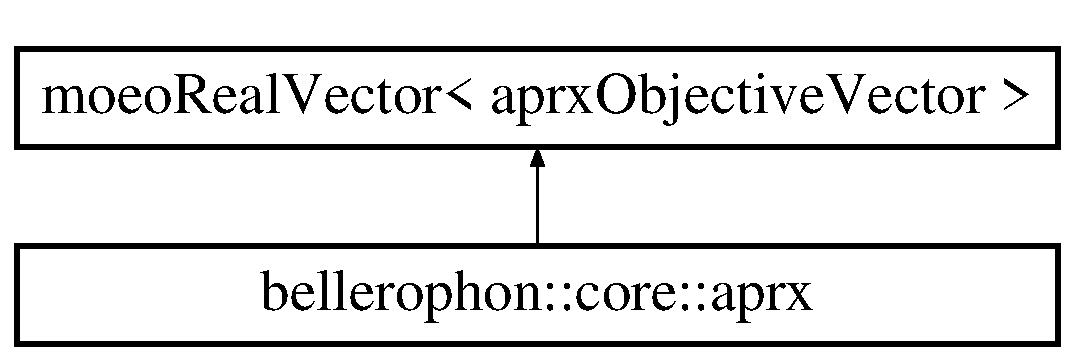
\includegraphics[height=2.000000cm]{classbellerophon_1_1core_1_1aprx}
\end{center}
\end{figure}
\subsection*{Public Member Functions}
\begin{DoxyCompactItemize}
\item 
\hypertarget{classbellerophon_1_1core_1_1aprx_aafee560c00eee20247dafa9a7a385c0e}{}\label{classbellerophon_1_1core_1_1aprx_aafee560c00eee20247dafa9a7a385c0e} 
{\bfseries aprx} (int n\+Aprx)
\item 
\hypertarget{classbellerophon_1_1core_1_1aprx_a1d11776015d1c42764bf30e7e627858a}{}\label{classbellerophon_1_1core_1_1aprx_a1d11776015d1c42764bf30e7e627858a} 
int {\bfseries get\+N\+Aprx} ()
\item 
\hypertarget{classbellerophon_1_1core_1_1aprx_a1c77803b9d4a481c81be2607bd1473dd}{}\label{classbellerophon_1_1core_1_1aprx_a1c77803b9d4a481c81be2607bd1473dd} 
void {\bfseries set\+N\+Aprx} (int n\+Aprx)
\end{DoxyCompactItemize}


The documentation for this class was generated from the following file\+:\begin{DoxyCompactItemize}
\item 
/home/ntonjeta/sharedfolder/bellerophon/include/\+Core/Evolution\+Context.\+h\end{DoxyCompactItemize}

\hypertarget{classbellerophon_1_1core_1_1AprxContext}{}\section{bellerophon\+:\+:core\+:\+:Aprx\+Context Class Reference}
\label{classbellerophon_1_1core_1_1AprxContext}\index{bellerophon\+::core\+::\+Aprx\+Context@{bellerophon\+::core\+::\+Aprx\+Context}}
Inheritance diagram for bellerophon\+:\+:core\+:\+:Aprx\+Context\+:\begin{figure}[H]
\begin{center}
\leavevmode
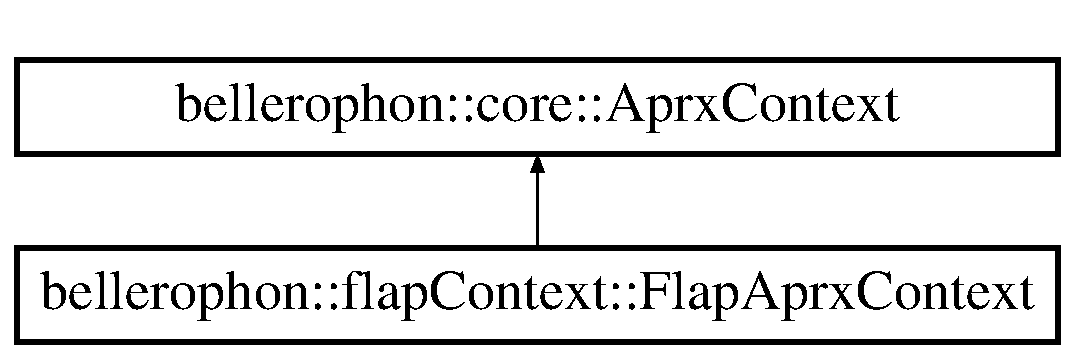
\includegraphics[height=2.000000cm]{classbellerophon_1_1core_1_1AprxContext}
\end{center}
\end{figure}
\subsection*{Public Member Functions}
\begin{DoxyCompactItemize}
\item 
\hypertarget{classbellerophon_1_1core_1_1AprxContext_a1311e2eae37a05fbb1c3afa166773ff7}{}\label{classbellerophon_1_1core_1_1AprxContext_a1311e2eae37a05fbb1c3afa166773ff7} 
{\bfseries Aprx\+Context} (Aprx\+Context\+Id\+Ty id, const \+::std\+::string \&desc)
\item 
\hypertarget{classbellerophon_1_1core_1_1AprxContext_a6e7500fec23c749aa7bed069443df135}{}\label{classbellerophon_1_1core_1_1AprxContext_a6e7500fec23c749aa7bed069443df135} 
Aprx\+Context\+Id\+Ty {\bfseries get\+Id} ()
\item 
\hypertarget{classbellerophon_1_1core_1_1AprxContext_a5da690361ab4810a2c27c7b733d513c3}{}\label{classbellerophon_1_1core_1_1AprxContext_a5da690361ab4810a2c27c7b733d513c3} 
\+::std\+::string {\bfseries get\+Desc} ()
\item 
\hypertarget{classbellerophon_1_1core_1_1AprxContext_a6d2fd57fea2a507cf0865f616516ea92}{}\label{classbellerophon_1_1core_1_1AprxContext_a6d2fd57fea2a507cf0865f616516ea92} 
Aprx\+Location\+Vector {\bfseries get\+Locations} ()
\item 
\hypertarget{classbellerophon_1_1core_1_1AprxContext_a9f5def40651b564a7d1fd71b85b7a03e}{}\label{classbellerophon_1_1core_1_1AprxContext_a9f5def40651b564a7d1fd71b85b7a03e} 
virtual \hyperlink{classbellerophon_1_1core_1_1AprxContext}{Aprx\+Context} $\ast$ {\bfseries operator=} (\hyperlink{classbellerophon_1_1core_1_1AprxContext}{Aprx\+Context} \&rhs)=0
\item 
\hypertarget{classbellerophon_1_1core_1_1AprxContext_aef2bb67ec7ac79c3f3a19f21d130ab17}{}\label{classbellerophon_1_1core_1_1AprxContext_aef2bb67ec7ac79c3f3a19f21d130ab17} 
void \hyperlink{classbellerophon_1_1core_1_1AprxContext_aef2bb67ec7ac79c3f3a19f21d130ab17}{add\+Location} (\+::std\+::shared\+\_\+ptr$<$ \hyperlink{classbellerophon_1_1core_1_1AprxTechnique}{Aprx\+Technique} $>$)
\begin{DoxyCompactList}\small\item\em Location mangment methods. \end{DoxyCompactList}\item 
\hypertarget{classbellerophon_1_1core_1_1AprxContext_a3376ace3532c7bb928eefd8d3220e1b4}{}\label{classbellerophon_1_1core_1_1AprxContext_a3376ace3532c7bb928eefd8d3220e1b4} 
void {\bfseries add\+Locations} (const \+::std\+::vector$<$\+::std\+::shared\+\_\+ptr$<$ \hyperlink{classbellerophon_1_1core_1_1AprxTechnique}{Aprx\+Technique} $>$$>$)
\item 
\hypertarget{classbellerophon_1_1core_1_1AprxContext_a0e7fcc06eb0b29d4196c2618b2d9f039}{}\label{classbellerophon_1_1core_1_1AprxContext_a0e7fcc06eb0b29d4196c2618b2d9f039} 
virtual void {\bfseries set\+Location} (const \+::std\+::vector$<$ \hyperlink{structbellerophon_1_1core_1_1AprxLocation}{Aprx\+Location} $>$)=0
\item 
void \hyperlink{classbellerophon_1_1core_1_1AprxContext_a3cbee10e05f6ef709f3663f2befff2db}{print\+Location} ()
\begin{DoxyCompactList}\small\item\em Add one location in Evolution Context. \end{DoxyCompactList}\item 
\hypertarget{classbellerophon_1_1core_1_1AprxContext_ae162fdaa857732bcf4f301e74bab102e}{}\label{classbellerophon_1_1core_1_1AprxContext_ae162fdaa857732bcf4f301e74bab102e} 
void {\bfseries print\+Location} (const Aprx\+Location\+Vector \&locations)
\item 
\hypertarget{classbellerophon_1_1core_1_1AprxContext_a27fa36a512613474ce79cf511ada6ad7}{}\label{classbellerophon_1_1core_1_1AprxContext_a27fa36a512613474ce79cf511ada6ad7} 
bool {\bfseries is\+Empty\+Loc} ()
\item 
virtual bool \hyperlink{classbellerophon_1_1core_1_1AprxContext_a6f7863e6f7d7146807247dca43a5af28}{read\+Report} (\+::std\+::string report)=0
\begin{DoxyCompactList}\small\item\em Virtual Method read report  Read approximation report generated by clang-\/chimera tools. \end{DoxyCompactList}\end{DoxyCompactItemize}
\subsection*{Protected Attributes}
\begin{DoxyCompactItemize}
\item 
\hypertarget{classbellerophon_1_1core_1_1AprxContext_a36cf8457115e90400323c0a248f0262e}{}\label{classbellerophon_1_1core_1_1AprxContext_a36cf8457115e90400323c0a248f0262e} 
Aprx\+Context\+Id\+Ty {\bfseries Id}
\item 
\hypertarget{classbellerophon_1_1core_1_1AprxContext_aef60cb2bc6d790594e34b56c526c8785}{}\label{classbellerophon_1_1core_1_1AprxContext_aef60cb2bc6d790594e34b56c526c8785} 
\+::std\+::string {\bfseries Desc}
\item 
\hypertarget{classbellerophon_1_1core_1_1AprxContext_aa41f847aae1a8673d11549aa8edcb89c}{}\label{classbellerophon_1_1core_1_1AprxContext_aa41f847aae1a8673d11549aa8edcb89c} 
Aprx\+Location\+Vector {\bfseries locations}
\end{DoxyCompactItemize}


\subsection{Member Function Documentation}
\hypertarget{classbellerophon_1_1core_1_1AprxContext_a3cbee10e05f6ef709f3663f2befff2db}{}\label{classbellerophon_1_1core_1_1AprxContext_a3cbee10e05f6ef709f3663f2befff2db} 
\index{bellerophon\+::core\+::\+Aprx\+Context@{bellerophon\+::core\+::\+Aprx\+Context}!print\+Location@{print\+Location}}
\index{print\+Location@{print\+Location}!bellerophon\+::core\+::\+Aprx\+Context@{bellerophon\+::core\+::\+Aprx\+Context}}
\subsubsection{\texorpdfstring{print\+Location()}{printLocation()}}
{\footnotesize\ttfamily void core\+::\+Aprx\+Context\+::print\+Location (\begin{DoxyParamCaption}{ }\end{DoxyParamCaption})}



Add one location in Evolution Context. 


\begin{DoxyParams}{Parameters}
{\em Aproximate\+Context} & instance \\
\hline
\end{DoxyParams}
\hypertarget{classbellerophon_1_1core_1_1AprxContext_a6f7863e6f7d7146807247dca43a5af28}{}\label{classbellerophon_1_1core_1_1AprxContext_a6f7863e6f7d7146807247dca43a5af28} 
\index{bellerophon\+::core\+::\+Aprx\+Context@{bellerophon\+::core\+::\+Aprx\+Context}!read\+Report@{read\+Report}}
\index{read\+Report@{read\+Report}!bellerophon\+::core\+::\+Aprx\+Context@{bellerophon\+::core\+::\+Aprx\+Context}}
\subsubsection{\texorpdfstring{read\+Report()}{readReport()}}
{\footnotesize\ttfamily virtual bool bellerophon\+::core\+::\+Aprx\+Context\+::read\+Report (\begin{DoxyParamCaption}\item[{\+::std\+::string}]{report }\end{DoxyParamCaption})\hspace{0.3cm}{\ttfamily [pure virtual]}}



Virtual Method read report  Read approximation report generated by clang-\/chimera tools. 

\begin{DoxyReturn}{Returns}
Return true if everything goes right 
\end{DoxyReturn}


Implemented in \hyperlink{classbellerophon_1_1flapContext_1_1FlapAprxContext_a3198868b5a8708c4976db9f1a70e70d5}{bellerophon\+::flap\+Context\+::\+Flap\+Aprx\+Context}.



The documentation for this class was generated from the following files\+:\begin{DoxyCompactItemize}
\item 
/home/ntonjeta/sharedfolder/bellerophon/include/\+Core/Aprx\+Context.\+h\item 
/home/ntonjeta/sharedfolder/bellerophon/src/\+Core/Aprx\+Context.\+cpp\end{DoxyCompactItemize}

\hypertarget{classbellerophon_1_1core_1_1aprxEval}{}\section{bellerophon\+:\+:core\+:\+:aprx\+Eval Class Reference}
\label{classbellerophon_1_1core_1_1aprxEval}\index{bellerophon\+::core\+::aprx\+Eval@{bellerophon\+::core\+::aprx\+Eval}}
Inheritance diagram for bellerophon\+:\+:core\+:\+:aprx\+Eval\+:\begin{figure}[H]
\begin{center}
\leavevmode
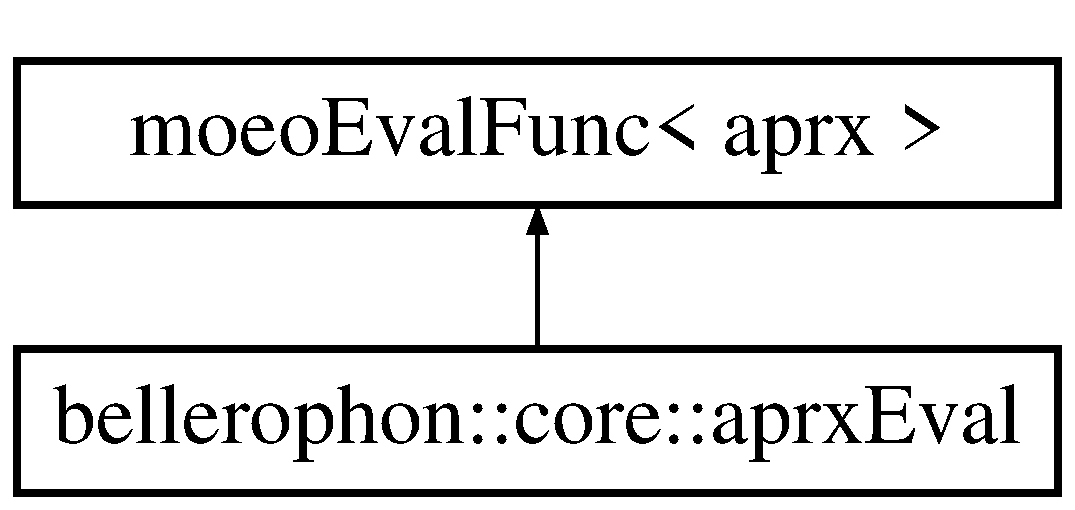
\includegraphics[height=2.000000cm]{classbellerophon_1_1core_1_1aprxEval}
\end{center}
\end{figure}
\subsection*{Public Member Functions}
\begin{DoxyCompactItemize}
\item 
\hypertarget{classbellerophon_1_1core_1_1aprxEval_abedbf814aa36df17b697246584f9e4b7}{}\label{classbellerophon_1_1core_1_1aprxEval_abedbf814aa36df17b697246584f9e4b7} 
void {\bfseries operator()} (\hyperlink{classbellerophon_1_1core_1_1aprx}{aprx} \&\+\_\+aprx)
\item 
\hypertarget{classbellerophon_1_1core_1_1aprxEval_a60bcda54bf5c58b5418d4560a30bdd48}{}\label{classbellerophon_1_1core_1_1aprxEval_a60bcda54bf5c58b5418d4560a30bdd48} 
int {\bfseries compile} ()
\item 
\hypertarget{classbellerophon_1_1core_1_1aprxEval_ad181047fea8b5b32e16786610c66de54}{}\label{classbellerophon_1_1core_1_1aprxEval_ad181047fea8b5b32e16786610c66de54} 
void {\bfseries set\+E\+E\+Helper} (\+::std\+::shared\+\_\+ptr$<$\+::\hyperlink{classbellerophon_1_1engine_1_1ExecutionEngineHelper}{bellerophon\+::engine\+::\+Execution\+Engine\+Helper} $>$ ee)
\item 
\hypertarget{classbellerophon_1_1core_1_1aprxEval_a6b4089083c46432709f42da00c5a10a1}{}\label{classbellerophon_1_1core_1_1aprxEval_a6b4089083c46432709f42da00c5a10a1} 
void {\bfseries set\+Aprx\+Loc} (const \+::bellerophon\+::core\+::\+Aprx\+Location\+Vector \&v)
\end{DoxyCompactItemize}


The documentation for this class was generated from the following files\+:\begin{DoxyCompactItemize}
\item 
/home/ntonjeta/sharedfolder/bellerophon/include/\+Core/Evolution\+Context.\+h\item 
/home/ntonjeta/sharedfolder/bellerophon/src/\+Core/Evolution\+Context.\+cpp\end{DoxyCompactItemize}

\hypertarget{structbellerophon_1_1core_1_1AprxLocation}{}\section{bellerophon\+:\+:core\+:\+:Aprx\+Location Struct Reference}
\label{structbellerophon_1_1core_1_1AprxLocation}\index{bellerophon\+::core\+::\+Aprx\+Location@{bellerophon\+::core\+::\+Aprx\+Location}}


Bind between an \hyperlink{classbellerophon_1_1core_1_1AprxTechnique}{Aprx\+Technique} and an aprx\+Grade that can be \textquotesingle{}accumulated\textquotesingle{}.  




{\ttfamily \#include $<$Aprx\+Context.\+h$>$}

\subsection*{Public Member Functions}
\begin{DoxyCompactItemize}
\item 
\hypertarget{structbellerophon_1_1core_1_1AprxLocation_a1639629d8fdc338b5f5fac77a954cbf0}{}\label{structbellerophon_1_1core_1_1AprxLocation_a1639629d8fdc338b5f5fac77a954cbf0} 
\hyperlink{structbellerophon_1_1core_1_1AprxLocation_a1639629d8fdc338b5f5fac77a954cbf0}{Aprx\+Location} (\+::std\+::shared\+\_\+ptr$<$ \hyperlink{classbellerophon_1_1core_1_1AprxTechnique}{Aprx\+Technique} $>$ t=nullptr, Aprx\+Grade grade=1)
\begin{DoxyCompactList}\small\item\em Constructor. \end{DoxyCompactList}\item 
\hypertarget{structbellerophon_1_1core_1_1AprxLocation_aac6ebc2d39f3991c9154134a9ff172bf}{}\label{structbellerophon_1_1core_1_1AprxLocation_aac6ebc2d39f3991c9154134a9ff172bf} 
\hyperlink{structbellerophon_1_1core_1_1AprxLocation}{Aprx\+Location} \hyperlink{structbellerophon_1_1core_1_1AprxLocation_aac6ebc2d39f3991c9154134a9ff172bf}{operator=} (const \hyperlink{structbellerophon_1_1core_1_1AprxLocation}{Aprx\+Location} \&rhs)
\begin{DoxyCompactList}\small\item\em Overloadin = operator. \end{DoxyCompactList}\end{DoxyCompactItemize}
\subsection*{Public Attributes}
\begin{DoxyCompactItemize}
\item 
\hypertarget{structbellerophon_1_1core_1_1AprxLocation_a70cbb151211e4bd36858030342234730}{}\label{structbellerophon_1_1core_1_1AprxLocation_a70cbb151211e4bd36858030342234730} 
\+::std\+::shared\+\_\+ptr$<$ \hyperlink{classbellerophon_1_1core_1_1AprxTechnique}{Aprx\+Technique} $>$ {\bfseries technique}
\item 
\hypertarget{structbellerophon_1_1core_1_1AprxLocation_a5916f0b3c29810d005a8a24e5c547ae5}{}\label{structbellerophon_1_1core_1_1AprxLocation_a5916f0b3c29810d005a8a24e5c547ae5} 
Aprx\+Grade {\bfseries g}
\end{DoxyCompactItemize}


\subsection{Detailed Description}
Bind between an \hyperlink{classbellerophon_1_1core_1_1AprxTechnique}{Aprx\+Technique} and an aprx\+Grade that can be \textquotesingle{}accumulated\textquotesingle{}. 

The documentation for this struct was generated from the following file\+:\begin{DoxyCompactItemize}
\item 
/home/ntonjeta/sharedfolder/bellerophon/include/\+Core/Aprx\+Context.\+h\end{DoxyCompactItemize}

\hypertarget{classbellerophon_1_1core_1_1AprxObjectiveVectorTraits}{}\section{bellerophon\+:\+:core\+:\+:Aprx\+Objective\+Vector\+Traits Class Reference}
\label{classbellerophon_1_1core_1_1AprxObjectiveVectorTraits}\index{bellerophon\+::core\+::\+Aprx\+Objective\+Vector\+Traits@{bellerophon\+::core\+::\+Aprx\+Objective\+Vector\+Traits}}
Inheritance diagram for bellerophon\+:\+:core\+:\+:Aprx\+Objective\+Vector\+Traits\+:\begin{figure}[H]
\begin{center}
\leavevmode
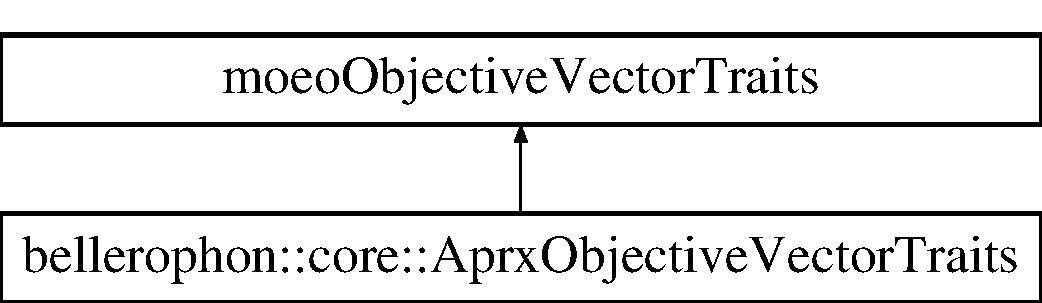
\includegraphics[height=2.000000cm]{classbellerophon_1_1core_1_1AprxObjectiveVectorTraits}
\end{center}
\end{figure}
\subsection*{Static Public Member Functions}
\begin{DoxyCompactItemize}
\item 
\hypertarget{classbellerophon_1_1core_1_1AprxObjectiveVectorTraits_a283aeb0cc76b497eae39234a595e4d8a}{}\label{classbellerophon_1_1core_1_1AprxObjectiveVectorTraits_a283aeb0cc76b497eae39234a595e4d8a} 
static bool {\bfseries minimizing} (int i)
\item 
\hypertarget{classbellerophon_1_1core_1_1AprxObjectiveVectorTraits_a6903dbc402df894a17277e6feb59bbcd}{}\label{classbellerophon_1_1core_1_1AprxObjectiveVectorTraits_a6903dbc402df894a17277e6feb59bbcd} 
static bool {\bfseries maximizing} (int i)
\item 
\hypertarget{classbellerophon_1_1core_1_1AprxObjectiveVectorTraits_a655781370e097ed2e9bab03f542a3b91}{}\label{classbellerophon_1_1core_1_1AprxObjectiveVectorTraits_a655781370e097ed2e9bab03f542a3b91} 
static unsigned int {\bfseries n\+Objectives} ()
\end{DoxyCompactItemize}


The documentation for this class was generated from the following file\+:\begin{DoxyCompactItemize}
\item 
/home/ntonjeta/sharedfolder/bellerophon/include/\+Core/Evolution\+Context.\+h\end{DoxyCompactItemize}

\hypertarget{classbellerophon_1_1core_1_1AprxTechnique}{}\section{bellerophon\+:\+:core\+:\+:Aprx\+Technique Class Reference}
\label{classbellerophon_1_1core_1_1AprxTechnique}\index{bellerophon\+::core\+::\+Aprx\+Technique@{bellerophon\+::core\+::\+Aprx\+Technique}}


Interface that abstracts an approximation strategy.  




{\ttfamily \#include $<$Aprx\+Technique.\+h$>$}

Inheritance diagram for bellerophon\+:\+:core\+:\+:Aprx\+Technique\+:\begin{figure}[H]
\begin{center}
\leavevmode
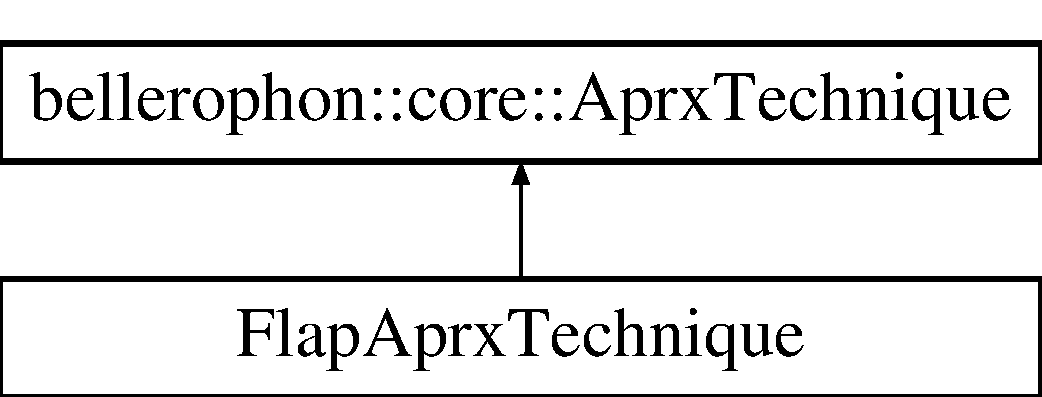
\includegraphics[height=2.000000cm]{classbellerophon_1_1core_1_1AprxTechnique}
\end{center}
\end{figure}
\subsection*{Public Member Functions}
\begin{DoxyCompactItemize}
\item 
\hypertarget{classbellerophon_1_1core_1_1AprxTechnique_ac495163cbd5c3479a425650f6a3c0371}{}\label{classbellerophon_1_1core_1_1AprxTechnique_ac495163cbd5c3479a425650f6a3c0371} 
{\bfseries Aprx\+Technique} (Aprx\+Technique\+Id\+Ty id)
\item 
\hypertarget{classbellerophon_1_1core_1_1AprxTechnique_a3afc9a467f5211a83d68b96014eff290}{}\label{classbellerophon_1_1core_1_1AprxTechnique_a3afc9a467f5211a83d68b96014eff290} 
Aprx\+Technique\+Id\+Ty {\bfseries get\+Id} () const
\item 
\hypertarget{classbellerophon_1_1core_1_1AprxTechnique_a655d22746c4cbe25f99599de1a299ff7}{}\label{classbellerophon_1_1core_1_1AprxTechnique_a655d22746c4cbe25f99599de1a299ff7} 
void {\bfseries set\+Id} (Aprx\+Technique\+Id\+Ty id)
\item 
virtual \+::std\+::vector$<$\+::std\+::string $>$ \hyperlink{classbellerophon_1_1core_1_1AprxTechnique_a834c99b86f8f9cdd1f411c685b36a275}{apply\+Approximation} (\+::bellerophon\+::core\+::\+Aprx\+Grade) const
\begin{DoxyCompactList}\small\item\em Apply an approximation. \end{DoxyCompactList}\item 
\hypertarget{classbellerophon_1_1core_1_1AprxTechnique_a797384b5484b0277f5268bbf4e23aa7c}{}\label{classbellerophon_1_1core_1_1AprxTechnique_a797384b5484b0277f5268bbf4e23aa7c} 
virtual void \hyperlink{classbellerophon_1_1core_1_1AprxTechnique_a797384b5484b0277f5268bbf4e23aa7c}{apply\+Approximation} (\+::bellerophon\+::core\+::\+Aprx\+Grade, \+::std\+::vector$<$ uint64\+\_\+t $>$) const =0
\begin{DoxyCompactList}\small\item\em Apply approximation using the addresses of variables. \end{DoxyCompactList}\item 
virtual \+::std\+::vector$<$\+::std\+::string $>$ \hyperlink{classbellerophon_1_1core_1_1AprxTechnique_a5d78bfe611a2e1884fd66f06ccde84d7}{get\+Global\+Value\+Names} () const
\begin{DoxyCompactList}\small\item\em Used with G\+L\+O\+B\+A\+L\+\_\+\+V\+A\+L\+U\+E\+\_\+\+M\+O\+D\+I\+F\+I\+C\+A\+T\+I\+ON approximation mode. \end{DoxyCompactList}\item 
virtual \+::bellerophon\+::core\+::\+Aprx\+Grade \hyperlink{classbellerophon_1_1core_1_1AprxTechnique_a6bcebd487e19b535ee4097d21f7df5db}{get\+Max\+Applicable\+Grade} () const =0
\begin{DoxyCompactList}\small\item\em Get the maximum approximation grade. \end{DoxyCompactList}\item 
\hypertarget{classbellerophon_1_1core_1_1AprxTechnique_a715a29fa676a36b3a96fbce5dbe1806b}{}\label{classbellerophon_1_1core_1_1AprxTechnique_a715a29fa676a36b3a96fbce5dbe1806b} 
virtual void \hyperlink{classbellerophon_1_1core_1_1AprxTechnique_a715a29fa676a36b3a96fbce5dbe1806b}{dump} (\+::llvm\+::raw\+\_\+ostream \&) const =0
\begin{DoxyCompactList}\small\item\em Dump information. \end{DoxyCompactList}\end{DoxyCompactItemize}
\subsection*{Protected Attributes}
\begin{DoxyCompactItemize}
\item 
\hypertarget{classbellerophon_1_1core_1_1AprxTechnique_a87301666e78094fc18da8b719b3d5bca}{}\label{classbellerophon_1_1core_1_1AprxTechnique_a87301666e78094fc18da8b719b3d5bca} 
Aprx\+Technique\+Id\+Ty {\bfseries Id}
\end{DoxyCompactItemize}


\subsection{Detailed Description}
Interface that abstracts an approximation strategy. 

It has to be implemented to create a context that is valid for an approximation strategy. 

\subsection{Member Function Documentation}
\hypertarget{classbellerophon_1_1core_1_1AprxTechnique_a834c99b86f8f9cdd1f411c685b36a275}{}\label{classbellerophon_1_1core_1_1AprxTechnique_a834c99b86f8f9cdd1f411c685b36a275} 
\index{bellerophon\+::core\+::\+Aprx\+Technique@{bellerophon\+::core\+::\+Aprx\+Technique}!apply\+Approximation@{apply\+Approximation}}
\index{apply\+Approximation@{apply\+Approximation}!bellerophon\+::core\+::\+Aprx\+Technique@{bellerophon\+::core\+::\+Aprx\+Technique}}
\subsubsection{\texorpdfstring{apply\+Approximation()}{applyApproximation()}}
{\footnotesize\ttfamily virtual \+::std\+::vector$<$\+::std\+::string$>$ bellerophon\+::core\+::\+Aprx\+Technique\+::apply\+Approximation (\begin{DoxyParamCaption}\item[{\+::bellerophon\+::core\+::\+Aprx\+Grade}]{ }\end{DoxyParamCaption}) const\hspace{0.3cm}{\ttfamily [inline]}}



Apply an approximation. 


\begin{DoxyParams}{Parameters}
{\em The} & approximation grade \\
\hline
\end{DoxyParams}
\begin{DoxyReturn}{Returns}
String vector containing compiler arguments that represent the approximation 
\end{DoxyReturn}
\hypertarget{classbellerophon_1_1core_1_1AprxTechnique_a5d78bfe611a2e1884fd66f06ccde84d7}{}\label{classbellerophon_1_1core_1_1AprxTechnique_a5d78bfe611a2e1884fd66f06ccde84d7} 
\index{bellerophon\+::core\+::\+Aprx\+Technique@{bellerophon\+::core\+::\+Aprx\+Technique}!get\+Global\+Value\+Names@{get\+Global\+Value\+Names}}
\index{get\+Global\+Value\+Names@{get\+Global\+Value\+Names}!bellerophon\+::core\+::\+Aprx\+Technique@{bellerophon\+::core\+::\+Aprx\+Technique}}
\subsubsection{\texorpdfstring{get\+Global\+Value\+Names()}{getGlobalValueNames()}}
{\footnotesize\ttfamily virtual \+::std\+::vector$<$\+::std\+::string$>$ bellerophon\+::core\+::\+Aprx\+Technique\+::get\+Global\+Value\+Names (\begin{DoxyParamCaption}{ }\end{DoxyParamCaption}) const\hspace{0.3cm}{\ttfamily [inline]}}



Used with G\+L\+O\+B\+A\+L\+\_\+\+V\+A\+L\+U\+E\+\_\+\+M\+O\+D\+I\+F\+I\+C\+A\+T\+I\+ON approximation mode. 

It provides the names of the global values that are required to be modified \hypertarget{classbellerophon_1_1core_1_1AprxTechnique_a6bcebd487e19b535ee4097d21f7df5db}{}\label{classbellerophon_1_1core_1_1AprxTechnique_a6bcebd487e19b535ee4097d21f7df5db} 
\index{bellerophon\+::core\+::\+Aprx\+Technique@{bellerophon\+::core\+::\+Aprx\+Technique}!get\+Max\+Applicable\+Grade@{get\+Max\+Applicable\+Grade}}
\index{get\+Max\+Applicable\+Grade@{get\+Max\+Applicable\+Grade}!bellerophon\+::core\+::\+Aprx\+Technique@{bellerophon\+::core\+::\+Aprx\+Technique}}
\subsubsection{\texorpdfstring{get\+Max\+Applicable\+Grade()}{getMaxApplicableGrade()}}
{\footnotesize\ttfamily virtual \+::bellerophon\+::core\+::\+Aprx\+Grade bellerophon\+::core\+::\+Aprx\+Technique\+::get\+Max\+Applicable\+Grade (\begin{DoxyParamCaption}{ }\end{DoxyParamCaption}) const\hspace{0.3cm}{\ttfamily [pure virtual]}}



Get the maximum approximation grade. 

\begin{DoxyReturn}{Returns}
Maximum approximation grade applicable 
\end{DoxyReturn}


Implemented in \hyperlink{classFlapAprxTechnique_af35c36c904e8c077c3fdf6bd35f5192c}{Flap\+Aprx\+Technique}.



The documentation for this class was generated from the following file\+:\begin{DoxyCompactItemize}
\item 
/home/ntonjeta/sharedfolder/bellerophon/include/\+Core/Aprx\+Technique.\+h\end{DoxyCompactItemize}

\hypertarget{classbellerophon_1_1log_1_1BellerophonLogger}{}\section{bellerophon\+:\+:log\+:\+:Bellerophon\+Logger Class Reference}
\label{classbellerophon_1_1log_1_1BellerophonLogger}\index{bellerophon\+::log\+::\+Bellerophon\+Logger@{bellerophon\+::log\+::\+Bellerophon\+Logger}}


Bellero\+Logger Class, provides all functions for the logging.  




{\ttfamily \#include $<$Log.\+h$>$}

\subsection*{Static Public Member Functions}
\begin{DoxyCompactItemize}
\item 
static void \hyperlink{classbellerophon_1_1log_1_1BellerophonLogger_a780401375c00ff261d6879d7ccf21861}{init} ()
\begin{DoxyCompactList}\small\item\em Initialize the logging class. \end{DoxyCompactList}\item 
\hypertarget{classbellerophon_1_1log_1_1BellerophonLogger_a63d06acba380395bebdfe777ff131997}{}\label{classbellerophon_1_1log_1_1BellerophonLogger_a63d06acba380395bebdfe777ff131997} 
static void \hyperlink{classbellerophon_1_1log_1_1BellerophonLogger_a63d06acba380395bebdfe777ff131997}{init\+Verbose} ()
\begin{DoxyCompactList}\small\item\em Enable the verbose level. \end{DoxyCompactList}\item 
\hypertarget{classbellerophon_1_1log_1_1BellerophonLogger_a60dfe793ccae33b38dc4871224455345}{}\label{classbellerophon_1_1log_1_1BellerophonLogger_a60dfe793ccae33b38dc4871224455345} 
static void \hyperlink{classbellerophon_1_1log_1_1BellerophonLogger_a60dfe793ccae33b38dc4871224455345}{init\+Trace} ()
\begin{DoxyCompactList}\small\item\em Enable the debug level. \end{DoxyCompactList}\item 
\hypertarget{classbellerophon_1_1log_1_1BellerophonLogger_af3b35d9d5d7f387e247b5ee0661a8e07}{}\label{classbellerophon_1_1log_1_1BellerophonLogger_af3b35d9d5d7f387e247b5ee0661a8e07} 
static void {\bfseries init} (int argc, const char $\ast$$\ast$argv)
\item 
\hypertarget{classbellerophon_1_1log_1_1BellerophonLogger_a9f42b16477dc255759e73a807c7bfaf6}{}\label{classbellerophon_1_1log_1_1BellerophonLogger_a9f42b16477dc255759e73a807c7bfaf6} 
static bool {\bfseries is\+Initialize} ()
\item 
\hypertarget{classbellerophon_1_1log_1_1BellerophonLogger_ad9c0de45f7a15044ded052122af255c2}{}\label{classbellerophon_1_1log_1_1BellerophonLogger_ad9c0de45f7a15044ded052122af255c2} 
static void {\bfseries set\+Verbose\+Level} (Verbose\+Level vlevel)
\item 
\hypertarget{classbellerophon_1_1log_1_1BellerophonLogger_a29d67e691ca3c1fa2eaa3ad57eebbb7e}{}\label{classbellerophon_1_1log_1_1BellerophonLogger_a29d67e691ca3c1fa2eaa3ad57eebbb7e} 
static void {\bfseries set\+Actual\+V\+Level} (Verbose\+Level vlevel)
\item 
\hypertarget{classbellerophon_1_1log_1_1BellerophonLogger_a9c929f62357eb9c14192640afa80edd5}{}\label{classbellerophon_1_1log_1_1BellerophonLogger_a9c929f62357eb9c14192640afa80edd5} 
static void {\bfseries reset\+Actual\+V\+Level} ()
\item 
\hypertarget{classbellerophon_1_1log_1_1BellerophonLogger_adc13b6d6b48df5c256881b55bf6c3824}{}\label{classbellerophon_1_1log_1_1BellerophonLogger_adc13b6d6b48df5c256881b55bf6c3824} 
static void {\bfseries incr\+Actual\+V\+Level} ()
\item 
\hypertarget{classbellerophon_1_1log_1_1BellerophonLogger_a0bfc45fde13bb492ffe5da977d091bc9}{}\label{classbellerophon_1_1log_1_1BellerophonLogger_a0bfc45fde13bb492ffe5da977d091bc9} 
static void {\bfseries decr\+Actual\+V\+Level} ()
\item 
static void \hyperlink{classbellerophon_1_1log_1_1BellerophonLogger_ad498ff6881211ff767a187e149c6ef53}{verbose} (Verbose\+Level, const std\+::string \&msg)
\begin{DoxyCompactList}\small\item\em Log a message for the Verbose level. \end{DoxyCompactList}\item 
\hypertarget{classbellerophon_1_1log_1_1BellerophonLogger_a40e7889408f1aad39c98de0a1309a532}{}\label{classbellerophon_1_1log_1_1BellerophonLogger_a40e7889408f1aad39c98de0a1309a532} 
static void \hyperlink{classbellerophon_1_1log_1_1BellerophonLogger_a40e7889408f1aad39c98de0a1309a532}{verbose} (const std\+::string \&msg)
\begin{DoxyCompactList}\small\item\em Log a message in Verbose actual level. \end{DoxyCompactList}\item 
\hypertarget{classbellerophon_1_1log_1_1BellerophonLogger_a173f8c75a7279dbac4be17e917a53fa6}{}\label{classbellerophon_1_1log_1_1BellerophonLogger_a173f8c75a7279dbac4be17e917a53fa6} 
static void {\bfseries verbose} (const std\+::string \&\&msg)
\item 
\hypertarget{classbellerophon_1_1log_1_1BellerophonLogger_a7a7378a416ea9c09dc654d4f2828f3ec}{}\label{classbellerophon_1_1log_1_1BellerophonLogger_a7a7378a416ea9c09dc654d4f2828f3ec} 
static void {\bfseries verbose\+And\+Incr} (const std\+::string \&msg)
\item 
\hypertarget{classbellerophon_1_1log_1_1BellerophonLogger_a326d3902798758ba65913c3fc1126cae}{}\label{classbellerophon_1_1log_1_1BellerophonLogger_a326d3902798758ba65913c3fc1126cae} 
static void {\bfseries verbose\+And\+Incr} (const std\+::string \&\&msg)
\item 
\hypertarget{classbellerophon_1_1log_1_1BellerophonLogger_aeca792a5bdf4d2a3a01ad7f6c9e9117e}{}\label{classbellerophon_1_1log_1_1BellerophonLogger_aeca792a5bdf4d2a3a01ad7f6c9e9117e} 
static void {\bfseries verbose\+And\+Decr} (const std\+::string \&msg)
\item 
\hypertarget{classbellerophon_1_1log_1_1BellerophonLogger_a2b6f45cbc14a4e2fecb98286ab7fa6e1}{}\label{classbellerophon_1_1log_1_1BellerophonLogger_a2b6f45cbc14a4e2fecb98286ab7fa6e1} 
static void {\bfseries verbose\+And\+Decr} (const std\+::string \&\&msg)
\item 
\hypertarget{classbellerophon_1_1log_1_1BellerophonLogger_a82ec294be519652ea15c950f659d3e2f}{}\label{classbellerophon_1_1log_1_1BellerophonLogger_a82ec294be519652ea15c950f659d3e2f} 
static void {\bfseries verbose\+Pre\+Decr} (const std\+::string \&msg)
\item 
\hypertarget{classbellerophon_1_1log_1_1BellerophonLogger_a9484408b0e87ccb04afc026093c14cb4}{}\label{classbellerophon_1_1log_1_1BellerophonLogger_a9484408b0e87ccb04afc026093c14cb4} 
static void {\bfseries verbose\+Pre\+Decr} (const std\+::string \&\&msg)
\item 
\hypertarget{classbellerophon_1_1log_1_1BellerophonLogger_adb4a8b2a17df0c6da35571fa26850d36}{}\label{classbellerophon_1_1log_1_1BellerophonLogger_adb4a8b2a17df0c6da35571fa26850d36} 
static void {\bfseries debug} (const std\+::string \&msg)
\item 
\hypertarget{classbellerophon_1_1log_1_1BellerophonLogger_a0ef2e0d50b2a30b9d980f3dc4fcae41a}{}\label{classbellerophon_1_1log_1_1BellerophonLogger_a0ef2e0d50b2a30b9d980f3dc4fcae41a} 
static void {\bfseries debug} (const std\+::string \&\&msg)
\item 
\hypertarget{classbellerophon_1_1log_1_1BellerophonLogger_a4787742f03add5f9fa92f4c395a0fc59}{}\label{classbellerophon_1_1log_1_1BellerophonLogger_a4787742f03add5f9fa92f4c395a0fc59} 
static void {\bfseries info} (const std\+::string \&msg)
\item 
\hypertarget{classbellerophon_1_1log_1_1BellerophonLogger_a475efbcf3cf3e20c34707ec75a5b4b59}{}\label{classbellerophon_1_1log_1_1BellerophonLogger_a475efbcf3cf3e20c34707ec75a5b4b59} 
static void {\bfseries info} (const std\+::string \&\&msg)
\item 
\hypertarget{classbellerophon_1_1log_1_1BellerophonLogger_ae9f80d59781394f85ff940f877b45130}{}\label{classbellerophon_1_1log_1_1BellerophonLogger_ae9f80d59781394f85ff940f877b45130} 
static void {\bfseries trace} (const std\+::string \&msg)
\item 
\hypertarget{classbellerophon_1_1log_1_1BellerophonLogger_a96aad2634d0c3338abd27f49fbbbe668}{}\label{classbellerophon_1_1log_1_1BellerophonLogger_a96aad2634d0c3338abd27f49fbbbe668} 
static void {\bfseries trace} (const std\+::string \&\&msg)
\item 
\hypertarget{classbellerophon_1_1log_1_1BellerophonLogger_ab7adf7e483d7a4f30a16331a65161efc}{}\label{classbellerophon_1_1log_1_1BellerophonLogger_ab7adf7e483d7a4f30a16331a65161efc} 
static void {\bfseries warning} (const std\+::string \&msg)
\item 
\hypertarget{classbellerophon_1_1log_1_1BellerophonLogger_a5e23b3d06515dc2610660646e6c99f03}{}\label{classbellerophon_1_1log_1_1BellerophonLogger_a5e23b3d06515dc2610660646e6c99f03} 
static void {\bfseries warning} (const std\+::string \&\&msg)
\item 
\hypertarget{classbellerophon_1_1log_1_1BellerophonLogger_a41a6707e911c46c3a78df45730cc6e95}{}\label{classbellerophon_1_1log_1_1BellerophonLogger_a41a6707e911c46c3a78df45730cc6e95} 
static void {\bfseries error} (const std\+::string \&msg)
\item 
\hypertarget{classbellerophon_1_1log_1_1BellerophonLogger_a0586f437126dbc33643e2c71ac1f6b4d}{}\label{classbellerophon_1_1log_1_1BellerophonLogger_a0586f437126dbc33643e2c71ac1f6b4d} 
static void {\bfseries error} (const std\+::string \&\&msg)
\item 
\hypertarget{classbellerophon_1_1log_1_1BellerophonLogger_a6fd49014f6c333644f54aff87b35ec9e}{}\label{classbellerophon_1_1log_1_1BellerophonLogger_a6fd49014f6c333644f54aff87b35ec9e} 
static void {\bfseries fatal} (const std\+::string \&msg)
\item 
\hypertarget{classbellerophon_1_1log_1_1BellerophonLogger_aace4d0e2028aa4464374053c6c558490}{}\label{classbellerophon_1_1log_1_1BellerophonLogger_aace4d0e2028aa4464374053c6c558490} 
static void {\bfseries fatal} (const std\+::string \&\&msg)
\end{DoxyCompactItemize}


\subsection{Detailed Description}
Bellero\+Logger Class, provides all functions for the logging. 

Through this helper class, it\textquotesingle{}s simpler to use easylogging++. 

\subsection{Member Function Documentation}
\hypertarget{classbellerophon_1_1log_1_1BellerophonLogger_a780401375c00ff261d6879d7ccf21861}{}\label{classbellerophon_1_1log_1_1BellerophonLogger_a780401375c00ff261d6879d7ccf21861} 
\index{bellerophon\+::log\+::\+Bellerophon\+Logger@{bellerophon\+::log\+::\+Bellerophon\+Logger}!init@{init}}
\index{init@{init}!bellerophon\+::log\+::\+Bellerophon\+Logger@{bellerophon\+::log\+::\+Bellerophon\+Logger}}
\subsubsection{\texorpdfstring{init()}{init()}}
{\footnotesize\ttfamily void log\+::\+Bellerophon\+Logger\+::init (\begin{DoxyParamCaption}{ }\end{DoxyParamCaption})\hspace{0.3cm}{\ttfamily [static]}}



Initialize the logging class. 

Configure el++ \+: chimera\+Logger \hypertarget{classbellerophon_1_1log_1_1BellerophonLogger_ad498ff6881211ff767a187e149c6ef53}{}\label{classbellerophon_1_1log_1_1BellerophonLogger_ad498ff6881211ff767a187e149c6ef53} 
\index{bellerophon\+::log\+::\+Bellerophon\+Logger@{bellerophon\+::log\+::\+Bellerophon\+Logger}!verbose@{verbose}}
\index{verbose@{verbose}!bellerophon\+::log\+::\+Bellerophon\+Logger@{bellerophon\+::log\+::\+Bellerophon\+Logger}}
\subsubsection{\texorpdfstring{verbose()}{verbose()}}
{\footnotesize\ttfamily void log\+::\+Bellerophon\+Logger\+::verbose (\begin{DoxyParamCaption}\item[{Verbose\+Level}]{vlevel,  }\item[{const std\+::string \&}]{msg }\end{DoxyParamCaption})\hspace{0.3cm}{\ttfamily [static]}}



Log a message for the Verbose level. 

Verbose levels are from 0 to 9 

The documentation for this class was generated from the following files\+:\begin{DoxyCompactItemize}
\item 
/home/ntonjeta/sharedfolder/bellerophon/include/\hyperlink{Log_8h}{Log.\+h}\item 
/home/ntonjeta/sharedfolder/bellerophon/src/\hyperlink{Log_8cpp}{Log.\+cpp}\end{DoxyCompactItemize}

\hypertarget{classbellerophon_1_1tool_1_1BellerophonTool}{}\section{bellerophon\+:\+:tool\+:\+:Bellerophon\+Tool Class Reference}
\label{classbellerophon_1_1tool_1_1BellerophonTool}\index{bellerophon\+::tool\+::\+Bellerophon\+Tool@{bellerophon\+::tool\+::\+Bellerophon\+Tool}}
\subsection*{Public Member Functions}
\begin{DoxyCompactItemize}
\item 
bool \hyperlink{classbellerophon_1_1tool_1_1BellerophonTool_aa10f85c0047eae4a7c2873995a9374f1}{register\+Aprx\+Context} (\+::std\+::shared\+\_\+ptr$<$ \hyperlink{classbellerophon_1_1core_1_1AprxContext}{bellerophon\+::core\+::\+Aprx\+Context} $>$)
\begin{DoxyCompactList}\small\item\em Register a Aprx\+Context. \end{DoxyCompactList}\item 
bool \hyperlink{classbellerophon_1_1tool_1_1BellerophonTool_abc426eaa463291b1f431e6c24c73c80e}{unregister\+Aprx\+Context} (const bellerophon\+::core\+::\+Aprx\+Context\+Id\+Ty \&)
\begin{DoxyCompactList}\small\item\em Unregister a aprx\+Context. \end{DoxyCompactList}\item 
\hypertarget{classbellerophon_1_1tool_1_1BellerophonTool_afe04397aa4e7b73185496f9c70c785a4}{}\label{classbellerophon_1_1tool_1_1BellerophonTool_afe04397aa4e7b73185496f9c70c785a4} 
void {\bfseries run} (int argc, const char $\ast$argv\mbox{[}$\,$\mbox{]})
\end{DoxyCompactItemize}


\subsection{Member Function Documentation}
\hypertarget{classbellerophon_1_1tool_1_1BellerophonTool_aa10f85c0047eae4a7c2873995a9374f1}{}\label{classbellerophon_1_1tool_1_1BellerophonTool_aa10f85c0047eae4a7c2873995a9374f1} 
\index{bellerophon\+::tool\+::\+Bellerophon\+Tool@{bellerophon\+::tool\+::\+Bellerophon\+Tool}!register\+Aprx\+Context@{register\+Aprx\+Context}}
\index{register\+Aprx\+Context@{register\+Aprx\+Context}!bellerophon\+::tool\+::\+Bellerophon\+Tool@{bellerophon\+::tool\+::\+Bellerophon\+Tool}}
\subsubsection{\texorpdfstring{register\+Aprx\+Context()}{registerAprxContext()}}
{\footnotesize\ttfamily bool tool\+::\+Bellerophon\+Tool\+::register\+Aprx\+Context (\begin{DoxyParamCaption}\item[{\+::std\+::shared\+\_\+ptr$<$ \hyperlink{classbellerophon_1_1core_1_1AprxContext}{bellerophon\+::core\+::\+Aprx\+Context} $>$}]{ }\end{DoxyParamCaption})}



Register a Aprx\+Context. 


\begin{DoxyParams}{Parameters}
{\em The} & Aprx\+Context to register \\
\hline
\end{DoxyParams}
\begin{DoxyReturn}{Returns}
If succeeded, if the operator\textquotesingle{}s identifier already exists the operation fails. 
\end{DoxyReturn}
\hypertarget{classbellerophon_1_1tool_1_1BellerophonTool_abc426eaa463291b1f431e6c24c73c80e}{}\label{classbellerophon_1_1tool_1_1BellerophonTool_abc426eaa463291b1f431e6c24c73c80e} 
\index{bellerophon\+::tool\+::\+Bellerophon\+Tool@{bellerophon\+::tool\+::\+Bellerophon\+Tool}!unregister\+Aprx\+Context@{unregister\+Aprx\+Context}}
\index{unregister\+Aprx\+Context@{unregister\+Aprx\+Context}!bellerophon\+::tool\+::\+Bellerophon\+Tool@{bellerophon\+::tool\+::\+Bellerophon\+Tool}}
\subsubsection{\texorpdfstring{unregister\+Aprx\+Context()}{unregisterAprxContext()}}
{\footnotesize\ttfamily bool tool\+::\+Bellerophon\+Tool\+::unregister\+Aprx\+Context (\begin{DoxyParamCaption}\item[{const bellerophon\+::core\+::\+Aprx\+Context\+Id\+Ty \&}]{id }\end{DoxyParamCaption})}



Unregister a aprx\+Context. 


\begin{DoxyParams}{Parameters}
{\em The} & identifier of the aprx\+Context \\
\hline
\end{DoxyParams}
\begin{DoxyReturn}{Returns}
If succeeded, id est the operator was registered 
\end{DoxyReturn}


The documentation for this class was generated from the following files\+:\begin{DoxyCompactItemize}
\item 
/home/ntonjeta/sharedfolder/bellerophon/include/\+Tool/Bellerophon\+Tool.\+h\item 
/home/ntonjeta/sharedfolder/bellerophon/src/\+Tool/Bellerophon\+Tool.\+cpp\end{DoxyCompactItemize}

\hypertarget{classbellerophon_1_1core_1_1EvolutionContext}{}\section{bellerophon\+:\+:core\+:\+:Evolution\+Context Class Reference}
\label{classbellerophon_1_1core_1_1EvolutionContext}\index{bellerophon\+::core\+::\+Evolution\+Context@{bellerophon\+::core\+::\+Evolution\+Context}}
\subsection*{Public Member Functions}
\begin{DoxyCompactItemize}
\item 
bool \hyperlink{classbellerophon_1_1core_1_1EvolutionContext_aab5413234e99512ab0208539cf866a8a}{init\+Execution\+Engine} (const \+::std\+::string \&)
\begin{DoxyCompactList}\small\item\em Init function for the internal execution engine. \end{DoxyCompactList}\item 
int \hyperlink{classbellerophon_1_1core_1_1EvolutionContext_a13906d3491e042f84473f0b10283acdd}{initialize\+Aprx\+Context} (\+::std\+::string path)
\begin{DoxyCompactList}\small\item\em Initialize the Aproximate Context. \end{DoxyCompactList}\item 
void \hyperlink{classbellerophon_1_1core_1_1EvolutionContext_ad21ec88b2a31a98140b052dcb0352cc9}{initialize\+Evolution} (double tau)
\begin{DoxyCompactList}\small\item\em Initialize the Evolution Parameter. \end{DoxyCompactList}\item 
void \hyperlink{classbellerophon_1_1core_1_1EvolutionContext_a8ec4af08d2fa630cd1a6daa4e6400cc4}{add\+Obj} (const \+::std\+::string \&obj\+Path)
\begin{DoxyCompactList}\small\item\em Add an object that will be loaded. \end{DoxyCompactList}\item 
void \hyperlink{classbellerophon_1_1core_1_1EvolutionContext_aa100267fe3f388b794dfeb6d1c105c89}{print\+Result} ()
\begin{DoxyCompactList}\small\item\em Apply the evolution algorithm. \end{DoxyCompactList}\item 
\hypertarget{classbellerophon_1_1core_1_1EvolutionContext_a37196148355350b656ea458053a7f3be}{}\label{classbellerophon_1_1core_1_1EvolutionContext_a37196148355350b656ea458053a7f3be} 
void \hyperlink{classbellerophon_1_1core_1_1EvolutionContext_a37196148355350b656ea458053a7f3be}{set\+Aprx\+Context} (const \+::std\+::shared\+\_\+ptr$<$\+::\hyperlink{classbellerophon_1_1core_1_1AprxContext}{bellerophon\+::core\+::\+Aprx\+Context} $>$ C)
\begin{DoxyCompactList}\small\item\em Initialize the Aprx Context. \end{DoxyCompactList}\end{DoxyCompactItemize}


\subsection{Member Function Documentation}
\hypertarget{classbellerophon_1_1core_1_1EvolutionContext_a8ec4af08d2fa630cd1a6daa4e6400cc4}{}\label{classbellerophon_1_1core_1_1EvolutionContext_a8ec4af08d2fa630cd1a6daa4e6400cc4} 
\index{bellerophon\+::core\+::\+Evolution\+Context@{bellerophon\+::core\+::\+Evolution\+Context}!add\+Obj@{add\+Obj}}
\index{add\+Obj@{add\+Obj}!bellerophon\+::core\+::\+Evolution\+Context@{bellerophon\+::core\+::\+Evolution\+Context}}
\subsubsection{\texorpdfstring{add\+Obj()}{addObj()}}
{\footnotesize\ttfamily void bellerophon\+::core\+::\+Evolution\+Context\+::add\+Obj (\begin{DoxyParamCaption}\item[{const \+::std\+::string \&}]{obj\+Path }\end{DoxyParamCaption})\hspace{0.3cm}{\ttfamily [inline]}}



Add an object that will be loaded. 


\begin{DoxyParams}{Parameters}
{\em obj\+Path} & Path to the object \\
\hline
\end{DoxyParams}
\hypertarget{classbellerophon_1_1core_1_1EvolutionContext_aab5413234e99512ab0208539cf866a8a}{}\label{classbellerophon_1_1core_1_1EvolutionContext_aab5413234e99512ab0208539cf866a8a} 
\index{bellerophon\+::core\+::\+Evolution\+Context@{bellerophon\+::core\+::\+Evolution\+Context}!init\+Execution\+Engine@{init\+Execution\+Engine}}
\index{init\+Execution\+Engine@{init\+Execution\+Engine}!bellerophon\+::core\+::\+Evolution\+Context@{bellerophon\+::core\+::\+Evolution\+Context}}
\subsubsection{\texorpdfstring{init\+Execution\+Engine()}{initExecutionEngine()}}
{\footnotesize\ttfamily bool bellerophon\+::core\+::\+Evolution\+Context\+::init\+Execution\+Engine (\begin{DoxyParamCaption}\item[{const \+::std\+::string \&}]{cd\+Path }\end{DoxyParamCaption})}



Init function for the internal execution engine. 

Initialize the exectution Engine.


\begin{DoxyParams}{Parameters}
{\em Compilation\+Database.\+json} & path \\
\hline
\end{DoxyParams}
\hypertarget{classbellerophon_1_1core_1_1EvolutionContext_a13906d3491e042f84473f0b10283acdd}{}\label{classbellerophon_1_1core_1_1EvolutionContext_a13906d3491e042f84473f0b10283acdd} 
\index{bellerophon\+::core\+::\+Evolution\+Context@{bellerophon\+::core\+::\+Evolution\+Context}!initialize\+Aprx\+Context@{initialize\+Aprx\+Context}}
\index{initialize\+Aprx\+Context@{initialize\+Aprx\+Context}!bellerophon\+::core\+::\+Evolution\+Context@{bellerophon\+::core\+::\+Evolution\+Context}}
\subsubsection{\texorpdfstring{initialize\+Aprx\+Context()}{initializeAprxContext()}}
{\footnotesize\ttfamily int bellerophon\+::core\+::\+Evolution\+Context\+::initialize\+Aprx\+Context (\begin{DoxyParamCaption}\item[{\+::std\+::string}]{path }\end{DoxyParamCaption})}



Initialize the Aproximate Context. 


\begin{DoxyParams}{Parameters}
{\em report} & path \\
\hline
\end{DoxyParams}
\begin{DoxyReturn}{Returns}
Satus Code 
\end{DoxyReturn}
\hypertarget{classbellerophon_1_1core_1_1EvolutionContext_ad21ec88b2a31a98140b052dcb0352cc9}{}\label{classbellerophon_1_1core_1_1EvolutionContext_ad21ec88b2a31a98140b052dcb0352cc9} 
\index{bellerophon\+::core\+::\+Evolution\+Context@{bellerophon\+::core\+::\+Evolution\+Context}!initialize\+Evolution@{initialize\+Evolution}}
\index{initialize\+Evolution@{initialize\+Evolution}!bellerophon\+::core\+::\+Evolution\+Context@{bellerophon\+::core\+::\+Evolution\+Context}}
\subsubsection{\texorpdfstring{initialize\+Evolution()}{initializeEvolution()}}
{\footnotesize\ttfamily void bellerophon\+::core\+::\+Evolution\+Context\+::initialize\+Evolution (\begin{DoxyParamCaption}\item[{double}]{tau }\end{DoxyParamCaption})}



Initialize the Evolution Parameter. 

Initialize Evolution algorithm.


\begin{DoxyParams}{Parameters}
{\em path} & to parameter file  Initialize the Evolution Parameter from file specified by path \\
\hline
\end{DoxyParams}
\hypertarget{classbellerophon_1_1core_1_1EvolutionContext_aa100267fe3f388b794dfeb6d1c105c89}{}\label{classbellerophon_1_1core_1_1EvolutionContext_aa100267fe3f388b794dfeb6d1c105c89} 
\index{bellerophon\+::core\+::\+Evolution\+Context@{bellerophon\+::core\+::\+Evolution\+Context}!print\+Result@{print\+Result}}
\index{print\+Result@{print\+Result}!bellerophon\+::core\+::\+Evolution\+Context@{bellerophon\+::core\+::\+Evolution\+Context}}
\subsubsection{\texorpdfstring{print\+Result()}{printResult()}}
{\footnotesize\ttfamily void bellerophon\+::core\+::\+Evolution\+Context\+::print\+Result (\begin{DoxyParamCaption}{ }\end{DoxyParamCaption})}



Apply the evolution algorithm. 


\begin{DoxyParams}{Parameters}
{\em taa} & double value constraint for generate error \textbackslash{} brief Print the result of evolution algorithm \\
\hline
\end{DoxyParams}


The documentation for this class was generated from the following files\+:\begin{DoxyCompactItemize}
\item 
/home/ntonjeta/sharedfolder/bellerophon/include/\+Core/Evolution\+Context.\+h\item 
/home/ntonjeta/sharedfolder/bellerophon/src/\+Core/Evolution\+Context.\+cpp\end{DoxyCompactItemize}

\hypertarget{classbellerophon_1_1engine_1_1ExecutionEngineHelper}{}\section{bellerophon\+:\+:engine\+:\+:Execution\+Engine\+Helper Class Reference}
\label{classbellerophon_1_1engine_1_1ExecutionEngineHelper}\index{bellerophon\+::engine\+::\+Execution\+Engine\+Helper@{bellerophon\+::engine\+::\+Execution\+Engine\+Helper}}


Helper class to interact with the L\+L\+VM execution engine.  




{\ttfamily \#include $<$Execution\+Engine\+Helper.\+h$>$}

\subsection*{Public Member Functions}
\begin{DoxyCompactItemize}
\item 
\hypertarget{classbellerophon_1_1engine_1_1ExecutionEngineHelper_acda31a25becaba3afd19312f43df054d}{}\label{classbellerophon_1_1engine_1_1ExecutionEngineHelper_acda31a25becaba3afd19312f43df054d} 
\hyperlink{classbellerophon_1_1engine_1_1ExecutionEngineHelper_acda31a25becaba3afd19312f43df054d}{Execution\+Engine\+Helper} ()
\begin{DoxyCompactList}\small\item\em Default ctor. \end{DoxyCompactList}\end{DoxyCompactItemize}
{\bf }\par
\begin{DoxyCompactItemize}
\item 
bool \hyperlink{classbellerophon_1_1engine_1_1ExecutionEngineHelper_a8bd642f019fd83f13ad986d9a95245db}{load\+Module} (\+::std\+::unique\+\_\+ptr$<$\+::llvm\+::\+Module $>$ M)
\begin{DoxyCompactList}\small\item\em Add the module {\ttfamily M} to the current execution engine. If it doesn\textquotesingle{}t exist it is created. \end{DoxyCompactList}\item 
bool \hyperlink{classbellerophon_1_1engine_1_1ExecutionEngineHelper_a05a050cb41cc3bf48977f52300e3ae52}{set\+Compilation\+Database} (const \+::std\+::string \&path)
\begin{DoxyCompactList}\small\item\em Take the path to a compilation database and load its compile commands. \end{DoxyCompactList}\item 
bool \hyperlink{classbellerophon_1_1engine_1_1ExecutionEngineHelper_a630f6808c11ca5c1dca005836af9ed59}{has\+Compile\+Command} (\+::llvm\+::\+String\+Ref filename)
\begin{DoxyCompactList}\small\item\em Check if {\ttfamily filename} has a compile command among the internal ones. \end{DoxyCompactList}\item 
int \hyperlink{classbellerophon_1_1engine_1_1ExecutionEngineHelper_a9f68c7cf6f58e299de0a06d96ada4fb2}{run\+Function} (\+::llvm\+::\+Generic\+Value \&retval, \+::llvm\+::\+String\+Ref func\+Name, \+::llvm\+::\+Array\+Ref$<$\+::llvm\+::\+Generic\+Value $>$ args=\+::llvm\+::\+None)
\begin{DoxyCompactList}\small\item\em Given a function name defined somewhere in the source files of which the compilation database have the compile commands, execute it and eventually returns its value. \end{DoxyCompactList}\item 
\hypertarget{classbellerophon_1_1engine_1_1ExecutionEngineHelper_a27e7e4fb1ba23cc31f4ff5e4aa227aa7}{}\label{classbellerophon_1_1engine_1_1ExecutionEngineHelper_a27e7e4fb1ba23cc31f4ff5e4aa227aa7} 
int \hyperlink{classbellerophon_1_1engine_1_1ExecutionEngineHelper_a27e7e4fb1ba23cc31f4ff5e4aa227aa7}{compile\+And\+Run\+Function} (\+::llvm\+::\+Generic\+Value \&retval, \+::llvm\+::\+String\+Ref func\+Name, \+::llvm\+::\+Array\+Ref$<$\+::llvm\+::\+Generic\+Value $>$ args=\+::llvm\+::\+None)
\begin{DoxyCompactList}\small\item\em Same as run\+Function but it previous performs the compilation. \end{DoxyCompactList}\end{DoxyCompactItemize}

{\bf }\par
\begin{DoxyCompactItemize}
\item 
uint64\+\_\+t \hyperlink{classbellerophon_1_1engine_1_1ExecutionEngineHelper_a9b72393d74d77555c1306abbdd930007}{get\+Address} (\+::llvm\+::\+String\+Ref)
\begin{DoxyCompactList}\small\item\em Get the address of a global value. \end{DoxyCompactList}\end{DoxyCompactItemize}

{\bf }\par
\begin{DoxyCompactItemize}
\item 
\hypertarget{classbellerophon_1_1engine_1_1ExecutionEngineHelper_a3254d7988bab8088f8cc22d02348748d}{}\label{classbellerophon_1_1engine_1_1ExecutionEngineHelper_a3254d7988bab8088f8cc22d02348748d} 
void {\bfseries set\+Additional\+Args} (const \+::std\+::vector$<$\+::std\+::string $>$ \&additional\+Args)
\item 
\hypertarget{classbellerophon_1_1engine_1_1ExecutionEngineHelper_af81d949184ac251787d6ace27a126302}{}\label{classbellerophon_1_1engine_1_1ExecutionEngineHelper_af81d949184ac251787d6ace27a126302} 
void {\bfseries clear\+Additional\+Args} ()
\item 
\hypertarget{classbellerophon_1_1engine_1_1ExecutionEngineHelper_ab687776f25d2d1aa7bdb200bac479d7f}{}\label{classbellerophon_1_1engine_1_1ExecutionEngineHelper_ab687776f25d2d1aa7bdb200bac479d7f} 
void {\bfseries set\+Obj\+Paths} (const \+::std\+::vector$<$\+::std\+::string $>$ \&object\+Paths)
\item 
\hypertarget{classbellerophon_1_1engine_1_1ExecutionEngineHelper_a824596d478fccec3fd4d81a5dd4dba20}{}\label{classbellerophon_1_1engine_1_1ExecutionEngineHelper_a824596d478fccec3fd4d81a5dd4dba20} 
void {\bfseries add\+Obj\+Path} (const \+::std\+::string \&obj\+Path)
\item 
\hypertarget{classbellerophon_1_1engine_1_1ExecutionEngineHelper_a555b5658918f2a14cbb03062531fdc24}{}\label{classbellerophon_1_1engine_1_1ExecutionEngineHelper_a555b5658918f2a14cbb03062531fdc24} 
void {\bfseries clear\+Obj\+Paths} ()
\item 
\hypertarget{classbellerophon_1_1engine_1_1ExecutionEngineHelper_ae256ea25e5844f8411911d5979af2a77}{}\label{classbellerophon_1_1engine_1_1ExecutionEngineHelper_ae256ea25e5844f8411911d5979af2a77} 
void {\bfseries set\+Archive\+Paths} (const \+::std\+::vector$<$\+::std\+::string $>$ \&paths)
\item 
\hypertarget{classbellerophon_1_1engine_1_1ExecutionEngineHelper_a741a12a635c41149af17fb291873ee73}{}\label{classbellerophon_1_1engine_1_1ExecutionEngineHelper_a741a12a635c41149af17fb291873ee73} 
void {\bfseries add\+Archive\+Path} (const \+::std\+::string \&path)
\item 
\hypertarget{classbellerophon_1_1engine_1_1ExecutionEngineHelper_ae6e8c69b6931c6a59e3baac42610f9d7}{}\label{classbellerophon_1_1engine_1_1ExecutionEngineHelper_ae6e8c69b6931c6a59e3baac42610f9d7} 
void {\bfseries clear\+Archive\+Paths} ()
\item 
\hypertarget{classbellerophon_1_1engine_1_1ExecutionEngineHelper_a002fdcd704a4b212aeba81b247f3740a}{}\label{classbellerophon_1_1engine_1_1ExecutionEngineHelper_a002fdcd704a4b212aeba81b247f3740a} 
void {\bfseries load\+Archive} (const \+::std\+::string \&path)
\item 
void \hyperlink{classbellerophon_1_1engine_1_1ExecutionEngineHelper_a6df2a721afdf41dab67487a9ac5ec9ba}{load\+Obj} (const \+::std\+::string \&obj\+Path)
\begin{DoxyCompactList}\small\item\em Load the objects contained in {\ttfamily obj\+Paths}. \end{DoxyCompactList}\item 
\hypertarget{classbellerophon_1_1engine_1_1ExecutionEngineHelper_a732a54bbac45e7df6e7afcf91bd7a8fd}{}\label{classbellerophon_1_1engine_1_1ExecutionEngineHelper_a732a54bbac45e7df6e7afcf91bd7a8fd} 
void {\bfseries load\+Objs} (const \+::std\+::vector$<$\+::std\+::string $>$ \&obj\+Paths)
\item 
\hypertarget{classbellerophon_1_1engine_1_1ExecutionEngineHelper_aad68e00a006a017fdfab64f7b8f8d366}{}\label{classbellerophon_1_1engine_1_1ExecutionEngineHelper_aad68e00a006a017fdfab64f7b8f8d366} 
int {\bfseries compile} ()
\end{DoxyCompactItemize}



\subsection{Detailed Description}
Helper class to interact with the L\+L\+VM execution engine. 

It manages a compilation database which contains the compile commands for a bunch of source files. These file can be compiled and linked in order to execute a function defined in them. At the moment is not supported the linking phase in which an external library can be specified. T\+O\+DO\+: Support libraries 

\subsection{Member Function Documentation}
\hypertarget{classbellerophon_1_1engine_1_1ExecutionEngineHelper_a9b72393d74d77555c1306abbdd930007}{}\label{classbellerophon_1_1engine_1_1ExecutionEngineHelper_a9b72393d74d77555c1306abbdd930007} 
\index{bellerophon\+::engine\+::\+Execution\+Engine\+Helper@{bellerophon\+::engine\+::\+Execution\+Engine\+Helper}!get\+Address@{get\+Address}}
\index{get\+Address@{get\+Address}!bellerophon\+::engine\+::\+Execution\+Engine\+Helper@{bellerophon\+::engine\+::\+Execution\+Engine\+Helper}}
\subsubsection{\texorpdfstring{get\+Address()}{getAddress()}}
{\footnotesize\ttfamily uint64\+\_\+t bellerophon\+::engine\+::\+Execution\+Engine\+Helper\+::get\+Address (\begin{DoxyParamCaption}\item[{\+::llvm\+::\+String\+Ref}]{Name }\end{DoxyParamCaption})}



Get the address of a global value. 

\begin{DoxyReturn}{Returns}
Equals to 0 if not founf 
\end{DoxyReturn}
\hypertarget{classbellerophon_1_1engine_1_1ExecutionEngineHelper_a630f6808c11ca5c1dca005836af9ed59}{}\label{classbellerophon_1_1engine_1_1ExecutionEngineHelper_a630f6808c11ca5c1dca005836af9ed59} 
\index{bellerophon\+::engine\+::\+Execution\+Engine\+Helper@{bellerophon\+::engine\+::\+Execution\+Engine\+Helper}!has\+Compile\+Command@{has\+Compile\+Command}}
\index{has\+Compile\+Command@{has\+Compile\+Command}!bellerophon\+::engine\+::\+Execution\+Engine\+Helper@{bellerophon\+::engine\+::\+Execution\+Engine\+Helper}}
\subsubsection{\texorpdfstring{has\+Compile\+Command()}{hasCompileCommand()}}
{\footnotesize\ttfamily bool bellerophon\+::engine\+::\+Execution\+Engine\+Helper\+::has\+Compile\+Command (\begin{DoxyParamCaption}\item[{\+::llvm\+::\+String\+Ref}]{filename }\end{DoxyParamCaption})}



Check if {\ttfamily filename} has a compile command among the internal ones. 


\begin{DoxyParams}{Parameters}
{\em filename} & The name of the file that should have a compile command \\
\hline
\end{DoxyParams}
\begin{DoxyReturn}{Returns}
If {\ttfamily filename} has a compile command 
\end{DoxyReturn}
\hypertarget{classbellerophon_1_1engine_1_1ExecutionEngineHelper_a8bd642f019fd83f13ad986d9a95245db}{}\label{classbellerophon_1_1engine_1_1ExecutionEngineHelper_a8bd642f019fd83f13ad986d9a95245db} 
\index{bellerophon\+::engine\+::\+Execution\+Engine\+Helper@{bellerophon\+::engine\+::\+Execution\+Engine\+Helper}!load\+Module@{load\+Module}}
\index{load\+Module@{load\+Module}!bellerophon\+::engine\+::\+Execution\+Engine\+Helper@{bellerophon\+::engine\+::\+Execution\+Engine\+Helper}}
\subsubsection{\texorpdfstring{load\+Module()}{loadModule()}}
{\footnotesize\ttfamily bool bellerophon\+::engine\+::\+Execution\+Engine\+Helper\+::load\+Module (\begin{DoxyParamCaption}\item[{\+::std\+::unique\+\_\+ptr$<$\+::llvm\+::\+Module $>$}]{M }\end{DoxyParamCaption})}



Add the module {\ttfamily M} to the current execution engine. If it doesn\textquotesingle{}t exist it is created. 


\begin{DoxyParams}{Parameters}
{\em M} & A L\+L\+VM Module \\
\hline
\end{DoxyParams}
\begin{DoxyReturn}{Returns}
If the set succeeds 
\end{DoxyReturn}
\hypertarget{classbellerophon_1_1engine_1_1ExecutionEngineHelper_a6df2a721afdf41dab67487a9ac5ec9ba}{}\label{classbellerophon_1_1engine_1_1ExecutionEngineHelper_a6df2a721afdf41dab67487a9ac5ec9ba} 
\index{bellerophon\+::engine\+::\+Execution\+Engine\+Helper@{bellerophon\+::engine\+::\+Execution\+Engine\+Helper}!load\+Obj@{load\+Obj}}
\index{load\+Obj@{load\+Obj}!bellerophon\+::engine\+::\+Execution\+Engine\+Helper@{bellerophon\+::engine\+::\+Execution\+Engine\+Helper}}
\subsubsection{\texorpdfstring{load\+Obj()}{loadObj()}}
{\footnotesize\ttfamily void bellerophon\+::engine\+::\+Execution\+Engine\+Helper\+::load\+Obj (\begin{DoxyParamCaption}\item[{const \+::std\+::string \&}]{obj\+Path }\end{DoxyParamCaption})}



Load the objects contained in {\ttfamily obj\+Paths}. 


\begin{DoxyParams}{Parameters}
{\em obj\+Paths} & Paths to object files \\
\hline
\end{DoxyParams}
\hypertarget{classbellerophon_1_1engine_1_1ExecutionEngineHelper_a9f68c7cf6f58e299de0a06d96ada4fb2}{}\label{classbellerophon_1_1engine_1_1ExecutionEngineHelper_a9f68c7cf6f58e299de0a06d96ada4fb2} 
\index{bellerophon\+::engine\+::\+Execution\+Engine\+Helper@{bellerophon\+::engine\+::\+Execution\+Engine\+Helper}!run\+Function@{run\+Function}}
\index{run\+Function@{run\+Function}!bellerophon\+::engine\+::\+Execution\+Engine\+Helper@{bellerophon\+::engine\+::\+Execution\+Engine\+Helper}}
\subsubsection{\texorpdfstring{run\+Function()}{runFunction()}}
{\footnotesize\ttfamily int bellerophon\+::engine\+::\+Execution\+Engine\+Helper\+::run\+Function (\begin{DoxyParamCaption}\item[{\+::llvm\+::\+Generic\+Value \&}]{retval,  }\item[{\+::llvm\+::\+String\+Ref}]{func\+Name,  }\item[{\+::llvm\+::\+Array\+Ref$<$\+::llvm\+::\+Generic\+Value $>$}]{args = {\ttfamily \+:\+:llvm\+:\+:None} }\end{DoxyParamCaption})}



Given a function name defined somewhere in the source files of which the compilation database have the compile commands, execute it and eventually returns its value. 

Using the J\+IT compiler of L\+L\+VM, the necessary files are just-\/in-\/time compiled, and then it is performed a linking phase and the {\ttfamily func\+Name} is executed passing {\ttfamily args} as arguments. 
\begin{DoxyParams}[1]{Parameters}
\mbox{\tt out}  & {\em retval} & Whatever the function returns \\
\hline
 & {\em func\+Name} & Name of the function to execute, it should be defined in the source files \\
\hline
 & {\em args} & Arguments to pass to the functions \\
\hline
\end{DoxyParams}
\begin{DoxyReturn}{Returns}
0 if succeeds, and then retval is properly set 1 otherwise 
\end{DoxyReturn}
\hypertarget{classbellerophon_1_1engine_1_1ExecutionEngineHelper_a05a050cb41cc3bf48977f52300e3ae52}{}\label{classbellerophon_1_1engine_1_1ExecutionEngineHelper_a05a050cb41cc3bf48977f52300e3ae52} 
\index{bellerophon\+::engine\+::\+Execution\+Engine\+Helper@{bellerophon\+::engine\+::\+Execution\+Engine\+Helper}!set\+Compilation\+Database@{set\+Compilation\+Database}}
\index{set\+Compilation\+Database@{set\+Compilation\+Database}!bellerophon\+::engine\+::\+Execution\+Engine\+Helper@{bellerophon\+::engine\+::\+Execution\+Engine\+Helper}}
\subsubsection{\texorpdfstring{set\+Compilation\+Database()}{setCompilationDatabase()}}
{\footnotesize\ttfamily bool bellerophon\+::engine\+::\+Execution\+Engine\+Helper\+::set\+Compilation\+Database (\begin{DoxyParamCaption}\item[{const \+::std\+::string \&}]{path }\end{DoxyParamCaption})}



Take the path to a compilation database and load its compile commands. 


\begin{DoxyParams}{Parameters}
{\em path} & Path to the dir in which there is the compilation database \\
\hline
\end{DoxyParams}
\begin{DoxyReturn}{Returns}
If the loading succeeds 
\end{DoxyReturn}


The documentation for this class was generated from the following files\+:\begin{DoxyCompactItemize}
\item 
/home/ntonjeta/sharedfolder/bellerophon/include/\+Execution\+Engine\+Helper/Execution\+Engine\+Helper.\+h\item 
/home/ntonjeta/sharedfolder/bellerophon/src/\+Execution\+Engine\+Helper/Execution\+Engine\+Helper.\+cpp\end{DoxyCompactItemize}

\hypertarget{classbellerophon_1_1flapContext_1_1FlapAprxContext}{}\section{bellerophon\+:\+:flap\+Context\+:\+:Flap\+Aprx\+Context Class Reference}
\label{classbellerophon_1_1flapContext_1_1FlapAprxContext}\index{bellerophon\+::flap\+Context\+::\+Flap\+Aprx\+Context@{bellerophon\+::flap\+Context\+::\+Flap\+Aprx\+Context}}
Inheritance diagram for bellerophon\+:\+:flap\+Context\+:\+:Flap\+Aprx\+Context\+:\begin{figure}[H]
\begin{center}
\leavevmode
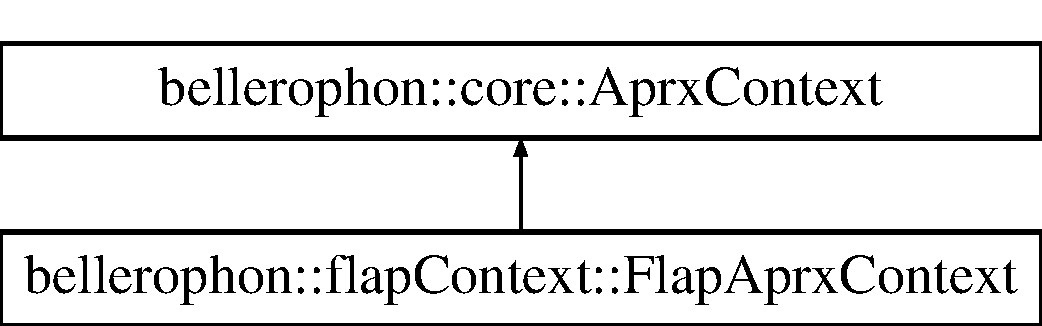
\includegraphics[height=2.000000cm]{classbellerophon_1_1flapContext_1_1FlapAprxContext}
\end{center}
\end{figure}
\subsection*{Public Member Functions}
\begin{DoxyCompactItemize}
\item 
\hypertarget{classbellerophon_1_1flapContext_1_1FlapAprxContext_a3db0cbccbefa15530deadffe922feebf}{}\label{classbellerophon_1_1flapContext_1_1FlapAprxContext_a3db0cbccbefa15530deadffe922feebf} 
{\bfseries Flap\+Aprx\+Context} (bellerophon\+::core\+::\+Aprx\+Context\+Id\+Ty id, const \+::std\+::string \&desc)
\item 
\hypertarget{classbellerophon_1_1flapContext_1_1FlapAprxContext_aea7d98ebcd3002914d32d69900866abd}{}\label{classbellerophon_1_1flapContext_1_1FlapAprxContext_aea7d98ebcd3002914d32d69900866abd} 
virtual void {\bfseries set\+Location} (\+::std\+::vector$<$ \hyperlink{structbellerophon_1_1core_1_1AprxLocation}{core\+::\+Aprx\+Location} $>$ tcqn) override
\item 
\hypertarget{classbellerophon_1_1flapContext_1_1FlapAprxContext_a4a523fe7bd877b30a1478a336565f058}{}\label{classbellerophon_1_1flapContext_1_1FlapAprxContext_a4a523fe7bd877b30a1478a336565f058} 
virtual \hyperlink{classbellerophon_1_1core_1_1AprxContext}{bellerophon\+::core\+::\+Aprx\+Context} $\ast$ {\bfseries operator=} (\hyperlink{classbellerophon_1_1core_1_1AprxContext}{bellerophon\+::core\+::\+Aprx\+Context} \&rhs) override
\item 
virtual bool \hyperlink{classbellerophon_1_1flapContext_1_1FlapAprxContext_a3198868b5a8708c4976db9f1a70e70d5}{read\+Report} (\+::std\+::string report) override
\begin{DoxyCompactList}\small\item\em Get the aprx locations for flap aprx techniques. \end{DoxyCompactList}\end{DoxyCompactItemize}
\subsection*{Additional Inherited Members}


\subsection{Member Function Documentation}
\hypertarget{classbellerophon_1_1flapContext_1_1FlapAprxContext_a3198868b5a8708c4976db9f1a70e70d5}{}\label{classbellerophon_1_1flapContext_1_1FlapAprxContext_a3198868b5a8708c4976db9f1a70e70d5} 
\index{bellerophon\+::flap\+Context\+::\+Flap\+Aprx\+Context@{bellerophon\+::flap\+Context\+::\+Flap\+Aprx\+Context}!read\+Report@{read\+Report}}
\index{read\+Report@{read\+Report}!bellerophon\+::flap\+Context\+::\+Flap\+Aprx\+Context@{bellerophon\+::flap\+Context\+::\+Flap\+Aprx\+Context}}
\subsubsection{\texorpdfstring{read\+Report()}{readReport()}}
{\footnotesize\ttfamily bool flap\+Context\+::\+Flap\+Aprx\+Context\+::read\+Report (\begin{DoxyParamCaption}\item[{\+::std\+::string}]{report }\end{DoxyParamCaption})\hspace{0.3cm}{\ttfamily [override]}, {\ttfamily [virtual]}}



Get the aprx locations for flap aprx techniques. 


\begin{DoxyParams}{Parameters}
{\em start\+Id} & The starting id for the contexts \\
\hline
{\em report\+Path} & The path to the report from which gather the info \\
\hline
\end{DoxyParams}
\begin{DoxyReturn}{Returns}
A vector of pointer to Flap\+Float\+Op\+Loc\+Context 
\end{DoxyReturn}


Implements \hyperlink{classbellerophon_1_1core_1_1AprxContext_a6f7863e6f7d7146807247dca43a5af28}{bellerophon\+::core\+::\+Aprx\+Context}.



The documentation for this class was generated from the following files\+:\begin{DoxyCompactItemize}
\item 
/home/ntonjeta/sharedfolder/bellerophon/include/\+Plugins/\+F\+L\+A\+P/Flap\+Aprx\+Context.\+h\item 
/home/ntonjeta/sharedfolder/bellerophon/src/\+Plugins/\+F\+L\+A\+P/Flap\+Aprx\+Context.\+cpp\end{DoxyCompactItemize}

\hypertarget{classFlapAprxTechnique}{}\section{Flap\+Aprx\+Technique Class Reference}
\label{classFlapAprxTechnique}\index{Flap\+Aprx\+Technique@{Flap\+Aprx\+Technique}}
Inheritance diagram for Flap\+Aprx\+Technique\+:\begin{figure}[H]
\begin{center}
\leavevmode
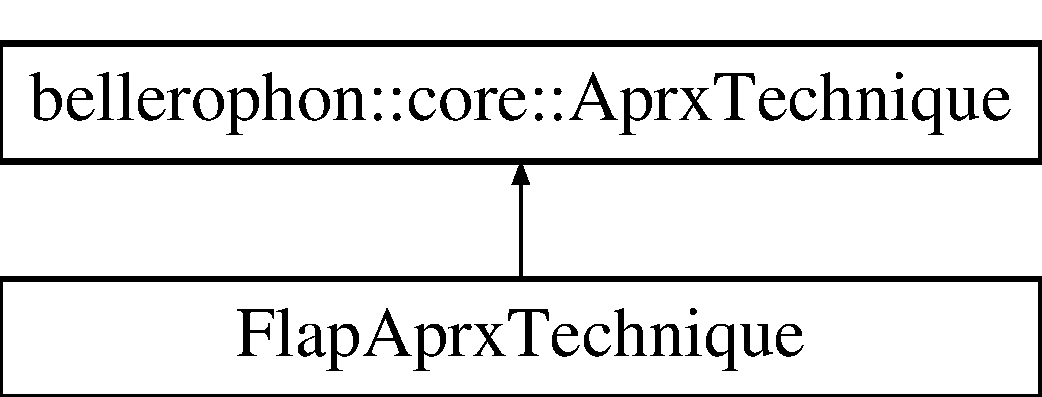
\includegraphics[height=2.000000cm]{classFlapAprxTechnique}
\end{center}
\end{figure}
\subsection*{Public Member Functions}
\begin{DoxyCompactItemize}
\item 
\hypertarget{classFlapAprxTechnique_aaf857d5880ae4252d4a2be9190728dde}{}\label{classFlapAprxTechnique_aaf857d5880ae4252d4a2be9190728dde} 
{\bfseries Flap\+Aprx\+Technique} (unsigned id, const \+::std\+::string op\+Id, Operation\+Ret\+Type rt\+Ty=F\+L\+O\+AT, Operation\+Type ty=A\+DD)
\item 
\hypertarget{classFlapAprxTechnique_aa5e7f37d6fd6559dcdae936173ecf7c0}{}\label{classFlapAprxTechnique_aa5e7f37d6fd6559dcdae936173ecf7c0} 
const \+::std\+::string \& {\bfseries get\+Op\+Id} () const
\item 
\hypertarget{classFlapAprxTechnique_a20a155653edc2ecb15a286ad20ad643c}{}\label{classFlapAprxTechnique_a20a155653edc2ecb15a286ad20ad643c} 
void {\bfseries set\+Op\+Id} (const \+::std\+::string \&op\+Id)
\item 
\hypertarget{classFlapAprxTechnique_a136c31fac2f58cd89a9fd9d4dbece992}{}\label{classFlapAprxTechnique_a136c31fac2f58cd89a9fd9d4dbece992} 
virtual \+::std\+::vector$<$\+::std\+::string $>$ {\bfseries get\+Global\+Value\+Names} () const override
\item 
\hypertarget{classFlapAprxTechnique_aefd2a4ab8d6ed9c92b34ff7860349590}{}\label{classFlapAprxTechnique_aefd2a4ab8d6ed9c92b34ff7860349590} 
virtual void \hyperlink{classFlapAprxTechnique_aefd2a4ab8d6ed9c92b34ff7860349590}{apply\+Approximation} (\+::bellerophon\+::core\+::\+Aprx\+Grade, \+::std\+::vector$<$ uint64\+\_\+t $>$) const override
\begin{DoxyCompactList}\small\item\em Apply approximation using the addresses of variables. \end{DoxyCompactList}\item 
\hypertarget{classFlapAprxTechnique_a93c20ee12acf2d5f12960706c12000ab}{}\label{classFlapAprxTechnique_a93c20ee12acf2d5f12960706c12000ab} 
virtual \+::std\+::vector$<$\+::std\+::string $>$ {\bfseries apply\+Approximation} (\+::bellerophon\+::core\+::\+Aprx\+Grade g) const override
\item 
virtual \+::bellerophon\+::core\+::\+Aprx\+Grade \hyperlink{classFlapAprxTechnique_af35c36c904e8c077c3fdf6bd35f5192c}{get\+Max\+Applicable\+Grade} () const override
\begin{DoxyCompactList}\small\item\em Get the maximum approximation grade. \end{DoxyCompactList}\item 
\hypertarget{classFlapAprxTechnique_a2d3dc7d3c0c44f6d49d51d2e460d298d}{}\label{classFlapAprxTechnique_a2d3dc7d3c0c44f6d49d51d2e460d298d} 
virtual void \hyperlink{classFlapAprxTechnique_a2d3dc7d3c0c44f6d49d51d2e460d298d}{dump} (\+::llvm\+::raw\+\_\+ostream \&out=\+::llvm\+::outs()) const override
\begin{DoxyCompactList}\small\item\em Dump information. \end{DoxyCompactList}\end{DoxyCompactItemize}
\subsection*{Public Attributes}
\begin{DoxyCompactItemize}
\item 
\hypertarget{classFlapAprxTechnique_a47a8663a3b30bd8c8236bc4d759df2ac}{}\label{classFlapAprxTechnique_a47a8663a3b30bd8c8236bc4d759df2ac} 
\+::std\+::string {\bfseries Operand\+L\+HS}
\item 
\hypertarget{classFlapAprxTechnique_a776f631a4c4fba99575c6251a9e5d645}{}\label{classFlapAprxTechnique_a776f631a4c4fba99575c6251a9e5d645} 
\+::std\+::string {\bfseries Operand\+R\+HS}
\end{DoxyCompactItemize}
\subsection*{Additional Inherited Members}


\subsection{Member Function Documentation}
\hypertarget{classFlapAprxTechnique_af35c36c904e8c077c3fdf6bd35f5192c}{}\label{classFlapAprxTechnique_af35c36c904e8c077c3fdf6bd35f5192c} 
\index{Flap\+Aprx\+Technique@{Flap\+Aprx\+Technique}!get\+Max\+Applicable\+Grade@{get\+Max\+Applicable\+Grade}}
\index{get\+Max\+Applicable\+Grade@{get\+Max\+Applicable\+Grade}!Flap\+Aprx\+Technique@{Flap\+Aprx\+Technique}}
\subsubsection{\texorpdfstring{get\+Max\+Applicable\+Grade()}{getMaxApplicableGrade()}}
{\footnotesize\ttfamily bellerophon\+::core\+::\+Aprx\+Grade Flap\+Aprx\+Technique\+::get\+Max\+Applicable\+Grade (\begin{DoxyParamCaption}{ }\end{DoxyParamCaption}) const\hspace{0.3cm}{\ttfamily [override]}, {\ttfamily [virtual]}}



Get the maximum approximation grade. 

\begin{DoxyReturn}{Returns}
Maximum approximation grade applicable 
\end{DoxyReturn}


Implements \hyperlink{classbellerophon_1_1core_1_1AprxTechnique_a6bcebd487e19b535ee4097d21f7df5db}{bellerophon\+::core\+::\+Aprx\+Technique}.



The documentation for this class was generated from the following files\+:\begin{DoxyCompactItemize}
\item 
/home/ntonjeta/sharedfolder/bellerophon/include/\+Plugins/\+F\+L\+A\+P/Flap\+Aprx\+Technique.\+h\item 
/home/ntonjeta/sharedfolder/bellerophon/src/\+Plugins/\+F\+L\+A\+P/Flap\+Aprx\+Technique.\+cpp\end{DoxyCompactItemize}

\hypertarget{classfap_1_1FloatingPointType}{}\section{fap\+:\+:Floating\+Point\+Type Class Reference}
\label{classfap_1_1FloatingPointType}\index{fap\+::\+Floating\+Point\+Type@{fap\+::\+Floating\+Point\+Type}}


Class for floating point type.  




{\ttfamily \#include $<$fap.\+h$>$}

\subsection*{Public Member Functions}
\begin{DoxyCompactItemize}
\item 
\hyperlink{classfap_1_1FloatingPointType_af4d0ebec7d0f2cff3e901a5a74a04d26}{operator float} () const
\begin{DoxyCompactList}\small\item\em brief Conversion to F\+A\+P\+\_\+fp\+\_\+t \end{DoxyCompactList}\item 
\hypertarget{classfap_1_1FloatingPointType_a7cac8cbb286a5a39a7afb475ea130db3}{}\label{classfap_1_1FloatingPointType_a7cac8cbb286a5a39a7afb475ea130db3} 
\hyperlink{classfap_1_1FloatingPointType_a7cac8cbb286a5a39a7afb475ea130db3}{operator double} () const
\begin{DoxyCompactList}\small\item\em brief Conversion to double \end{DoxyCompactList}\item 
\hypertarget{classfap_1_1FloatingPointType_ab6d80415c8b3752813362d0ec58b672a}{}\label{classfap_1_1FloatingPointType_ab6d80415c8b3752813362d0ec58b672a} 
\hyperlink{classfap_1_1FloatingPointType_ab6d80415c8b3752813362d0ec58b672a}{operator int} () const
\begin{DoxyCompactList}\small\item\em brief Conversion to int \end{DoxyCompactList}\item 
\hypertarget{classfap_1_1FloatingPointType_a206e802e7b114122b4baccd31576b0d1}{}\label{classfap_1_1FloatingPointType_a206e802e7b114122b4baccd31576b0d1} 
\hyperlink{classfap_1_1FloatingPointType_a206e802e7b114122b4baccd31576b0d1}{operator unsigned char} () const
\begin{DoxyCompactList}\small\item\em brief Conversion to unsigned char \end{DoxyCompactList}\item 
\hypertarget{classfap_1_1FloatingPointType_a6062aaca7b0271bbbb6eed490e1ad876}{}\label{classfap_1_1FloatingPointType_a6062aaca7b0271bbbb6eed490e1ad876} 
\hyperlink{classfap_1_1FloatingPointType}{Floating\+Point\+Type} \& {\bfseries operator=} (float)
\item 
\hypertarget{classfap_1_1FloatingPointType_ad151ca999715cc070983721da11a0365}{}\label{classfap_1_1FloatingPointType_ad151ca999715cc070983721da11a0365} 
\hyperlink{classfap_1_1FloatingPointType}{Floating\+Point\+Type} \& {\bfseries operator=} (double)
\item 
\hypertarget{classfap_1_1FloatingPointType_a5ca179a0e279471fb87cf97ed47defe9}{}\label{classfap_1_1FloatingPointType_a5ca179a0e279471fb87cf97ed47defe9} 
\hyperlink{classfap_1_1FloatingPointType}{Floating\+Point\+Type} \& {\bfseries operator=} (int i)
\item 
\hypertarget{classfap_1_1FloatingPointType_a01ed0f214cf97046a2179bc7ffcdc132}{}\label{classfap_1_1FloatingPointType_a01ed0f214cf97046a2179bc7ffcdc132} 
\hyperlink{classfap_1_1FloatingPointType}{Floating\+Point\+Type} \& {\bfseries operator+=} (const \hyperlink{classfap_1_1FloatingPointType}{Floating\+Point\+Type} \&fp)
\item 
\hypertarget{classfap_1_1FloatingPointType_abdd7ac11001e25e57b0288462f134914}{}\label{classfap_1_1FloatingPointType_abdd7ac11001e25e57b0288462f134914} 
\hyperlink{classfap_1_1FloatingPointType}{Floating\+Point\+Type} \& {\bfseries operator-\/=} (const \hyperlink{classfap_1_1FloatingPointType}{Floating\+Point\+Type} \&fp)
\item 
\hypertarget{classfap_1_1FloatingPointType_afdfc256b91a4a21b3d909c176e6ed3f5}{}\label{classfap_1_1FloatingPointType_afdfc256b91a4a21b3d909c176e6ed3f5} 
\hyperlink{classfap_1_1FloatingPointType}{Floating\+Point\+Type} \& {\bfseries operator$\ast$=} (const \hyperlink{classfap_1_1FloatingPointType}{Floating\+Point\+Type} \&fp)
\item 
\hypertarget{classfap_1_1FloatingPointType_a1c2960c105ce9f49dd6249fa1c41ae25}{}\label{classfap_1_1FloatingPointType_a1c2960c105ce9f49dd6249fa1c41ae25} 
\hyperlink{classfap_1_1FloatingPointType}{Floating\+Point\+Type} \& {\bfseries operator/=} (const \hyperlink{classfap_1_1FloatingPointType}{Floating\+Point\+Type} \&fp)
\item 
\hypertarget{classfap_1_1FloatingPointType_a78f11f14da68bc3d04a563ae600f2e55}{}\label{classfap_1_1FloatingPointType_a78f11f14da68bc3d04a563ae600f2e55} 
bool {\bfseries operator$<$=} (const \hyperlink{classfap_1_1FloatingPointType}{Floating\+Point\+Type} \&rhs)
\item 
\hypertarget{classfap_1_1FloatingPointType_ac74a7b58dd4fff532e10affc83083ea1}{}\label{classfap_1_1FloatingPointType_ac74a7b58dd4fff532e10affc83083ea1} 
bool {\bfseries operator$<$} (const \hyperlink{classfap_1_1FloatingPointType}{Floating\+Point\+Type} \&rhs)
\item 
\hypertarget{classfap_1_1FloatingPointType_a8ad1366a3b349973923fd84bd762c0b2}{}\label{classfap_1_1FloatingPointType_a8ad1366a3b349973923fd84bd762c0b2} 
bool {\bfseries operator$>$=} (const \hyperlink{classfap_1_1FloatingPointType}{Floating\+Point\+Type} \&rhs)
\item 
\hypertarget{classfap_1_1FloatingPointType_ac42658174f0d455de56829781c1d3558}{}\label{classfap_1_1FloatingPointType_ac42658174f0d455de56829781c1d3558} 
bool {\bfseries operator$>$} (const \hyperlink{classfap_1_1FloatingPointType}{Floating\+Point\+Type} \&rhs)
\item 
\hypertarget{classfap_1_1FloatingPointType_a1cbb93d976a0fe84fade02f77ec280e9}{}\label{classfap_1_1FloatingPointType_a1cbb93d976a0fe84fade02f77ec280e9} 
bool {\bfseries is\+Zero} () const
\item 
\hypertarget{classfap_1_1FloatingPointType_a528562ecb5fc3156ae9e36751a86b837}{}\label{classfap_1_1FloatingPointType_a528562ecb5fc3156ae9e36751a86b837} 
bool {\bfseries is\+SubN} () const
\item 
\hypertarget{classfap_1_1FloatingPointType_abc5d8c3cc037c4479552abb09218488f}{}\label{classfap_1_1FloatingPointType_abc5d8c3cc037c4479552abb09218488f} 
bool {\bfseries is\+Inf} () const
\item 
\hypertarget{classfap_1_1FloatingPointType_a14fa7dc64c182350d3818e8174e74ec5}{}\label{classfap_1_1FloatingPointType_a14fa7dc64c182350d3818e8174e74ec5} 
bool {\bfseries is\+Pinf} () const
\item 
\hypertarget{classfap_1_1FloatingPointType_aeb0bcea5139d560c5fc614a5f871bd3f}{}\label{classfap_1_1FloatingPointType_aeb0bcea5139d560c5fc614a5f871bd3f} 
bool {\bfseries is\+Ninf} () const
\item 
\hypertarget{classfap_1_1FloatingPointType_a93e5f9bee036086c80bbd31574d823ce}{}\label{classfap_1_1FloatingPointType_a93e5f9bee036086c80bbd31574d823ce} 
bool {\bfseries is\+NaN} () const
\item 
\hypertarget{classfap_1_1FloatingPointType_a2f0edab95a0adc795121c3ac3b4e16f8}{}\label{classfap_1_1FloatingPointType_a2f0edab95a0adc795121c3ac3b4e16f8} 
void {\bfseries set\+Zero} ()
\item 
\hypertarget{classfap_1_1FloatingPointType_a3c29014aadd2e23315b9ebaf76b7c56a}{}\label{classfap_1_1FloatingPointType_a3c29014aadd2e23315b9ebaf76b7c56a} 
void {\bfseries set\+Inf} ()
\item 
\hypertarget{classfap_1_1FloatingPointType_ad4a1f36aae890e6e004092e5d6d9e1f4}{}\label{classfap_1_1FloatingPointType_ad4a1f36aae890e6e004092e5d6d9e1f4} 
void {\bfseries set\+Pinf} ()
\item 
\hypertarget{classfap_1_1FloatingPointType_a7ef3600f368c55d2c26e6102464acbf0}{}\label{classfap_1_1FloatingPointType_a7ef3600f368c55d2c26e6102464acbf0} 
void {\bfseries set\+Ninf} ()
\item 
\hypertarget{classfap_1_1FloatingPointType_af00c1e36d1c917ac204cdfff10605fbf}{}\label{classfap_1_1FloatingPointType_af00c1e36d1c917ac204cdfff10605fbf} 
void {\bfseries set\+NaN} ()
\item 
\hypertarget{classfap_1_1FloatingPointType_a5f8d63229817025e70c8674c3c06c052}{}\label{classfap_1_1FloatingPointType_a5f8d63229817025e70c8674c3c06c052} 
void {\bfseries adapt\+Prec} (\hyperlink{classfap_1_1FloatingPointType}{Floating\+Point\+Type} \&)
\item 
\hypertarget{classfap_1_1FloatingPointType_abdad4f2a38b5764df31d14067e58541e}{}\label{classfap_1_1FloatingPointType_abdad4f2a38b5764df31d14067e58541e} 
void {\bfseries change\+Prec} (\hyperlink{structfap_1_1FloatPrecTy}{Float\+Prec\+Ty})
\item 
\hypertarget{classfap_1_1FloatingPointType_a720c3d8559a7c6639a1242f738ffb598}{}\label{classfap_1_1FloatingPointType_a720c3d8559a7c6639a1242f738ffb598} 
void {\bfseries shift} (int)
\item 
\hypertarget{classfap_1_1FloatingPointType_a09ecdb05d2d6df1c04241896dcf0d815}{}\label{classfap_1_1FloatingPointType_a09ecdb05d2d6df1c04241896dcf0d815} 
void {\bfseries normalize} (int, int)
\item 
\hypertarget{classfap_1_1FloatingPointType_a9398f79f15929853507657140b92f60f}{}\label{classfap_1_1FloatingPointType_a9398f79f15929853507657140b92f60f} 
void {\bfseries round} (F\+A\+P\+\_\+rounding\+\_\+method method=F\+A\+P\+\_\+\+F\+P\+\_\+\+R\+O\+U\+N\+D\+\_\+\+N\+E\+A\+R\+E\+ST)
\end{DoxyCompactItemize}
{\bf }\par
\begin{DoxyCompactItemize}
\item 
\hypertarget{classfap_1_1FloatingPointType_a7362ec3dd87a16389ead3199e1c69345}{}\label{classfap_1_1FloatingPointType_a7362ec3dd87a16389ead3199e1c69345} 
\hyperlink{classfap_1_1FloatingPointType_a7362ec3dd87a16389ead3199e1c69345}{Floating\+Point\+Type} ()
\begin{DoxyCompactList}\small\item\em Default ctor. \end{DoxyCompactList}\item 
\hyperlink{classfap_1_1FloatingPointType_aa89105fd5d48eb7165b2234f852c7a19}{Floating\+Point\+Type} (float f, \hyperlink{structfap_1_1FloatPrecTy}{Float\+Prec\+Ty} n\+\_\+prec=\{F\+L\+O\+A\+T\+\_\+\+E\+X\+P\+\_\+\+S\+I\+ZE, F\+L\+O\+A\+T\+\_\+\+M\+A\+N\+T\+\_\+\+S\+I\+ZE\})
\begin{DoxyCompactList}\small\item\em Conversion from F\+A\+P\+\_\+fp\+\_\+t. \end{DoxyCompactList}\item 
\hypertarget{classfap_1_1FloatingPointType_aa3b2a25eb533eab4b25f75f506947a50}{}\label{classfap_1_1FloatingPointType_aa3b2a25eb533eab4b25f75f506947a50} 
\hyperlink{classfap_1_1FloatingPointType_aa3b2a25eb533eab4b25f75f506947a50}{Floating\+Point\+Type} (double d, \hyperlink{structfap_1_1FloatPrecTy}{Float\+Prec\+Ty} n\+\_\+prec=\{D\+O\+U\+B\+L\+E\+\_\+\+E\+X\+P\+\_\+\+S\+I\+ZE, D\+O\+U\+B\+L\+E\+\_\+\+M\+A\+N\+T\+\_\+\+S\+I\+ZE\})
\begin{DoxyCompactList}\small\item\em Conversion from double. \end{DoxyCompactList}\item 
\hypertarget{classfap_1_1FloatingPointType_aef499a348920080ca3dbdc728977570a}{}\label{classfap_1_1FloatingPointType_aef499a348920080ca3dbdc728977570a} 
\hyperlink{classfap_1_1FloatingPointType_aef499a348920080ca3dbdc728977570a}{Floating\+Point\+Type} (int i, \hyperlink{structfap_1_1FloatPrecTy}{Float\+Prec\+Ty} n\+\_\+prec=\{D\+O\+U\+B\+L\+E\+\_\+\+E\+X\+P\+\_\+\+S\+I\+ZE, D\+O\+U\+B\+L\+E\+\_\+\+M\+A\+N\+T\+\_\+\+S\+I\+ZE\})
\begin{DoxyCompactList}\small\item\em Conversion from int. \end{DoxyCompactList}\end{DoxyCompactItemize}

{\bf }\par
\begin{DoxyCompactItemize}
\item 
\hypertarget{classfap_1_1FloatingPointType_a8edcfd0115d8a7cd90b9210b78724e94}{}\label{classfap_1_1FloatingPointType_a8edcfd0115d8a7cd90b9210b78724e94} 
Sign\+Type {\bfseries get\+Sign} () const
\item 
\hypertarget{classfap_1_1FloatingPointType_a1c7b069971075c7b7929ed00b221c735}{}\label{classfap_1_1FloatingPointType_a1c7b069971075c7b7929ed00b221c735} 
void {\bfseries set\+Sign} (Sign\+Type sign)
\item 
\hypertarget{classfap_1_1FloatingPointType_a9203127528e8c0b23039d1123c1a66bd}{}\label{classfap_1_1FloatingPointType_a9203127528e8c0b23039d1123c1a66bd} 
Exp\+Type {\bfseries get\+Exp} () const
\item 
\hypertarget{classfap_1_1FloatingPointType_a9b5e92f21d5ee59a6625715ff3aea55e}{}\label{classfap_1_1FloatingPointType_a9b5e92f21d5ee59a6625715ff3aea55e} 
void {\bfseries set\+Exp} (Exp\+Type exp)
\item 
\hypertarget{classfap_1_1FloatingPointType_a034b7c05ed25be51bff39718ef2dbf1b}{}\label{classfap_1_1FloatingPointType_a034b7c05ed25be51bff39718ef2dbf1b} 
Mant\+Type {\bfseries get\+Mant} () const
\item 
\hypertarget{classfap_1_1FloatingPointType_aec79acfef5ff08ec9bb1b12fb95f2e48}{}\label{classfap_1_1FloatingPointType_aec79acfef5ff08ec9bb1b12fb95f2e48} 
void {\bfseries set\+Mant} (Mant\+Type mant)
\item 
\hypertarget{classfap_1_1FloatingPointType_a4fa0e0aea038147ef314efe3e7686e7d}{}\label{classfap_1_1FloatingPointType_a4fa0e0aea038147ef314efe3e7686e7d} 
Mant\+Type {\bfseries get\+Mant\+Hb} () const
\item 
\hypertarget{classfap_1_1FloatingPointType_a542075e72b8f5a3642591d1e76927d77}{}\label{classfap_1_1FloatingPointType_a542075e72b8f5a3642591d1e76927d77} 
void {\bfseries set\+Mant\+Hb} ()
\item 
\hypertarget{classfap_1_1FloatingPointType_a024eabd2fb98379f0486f4f2e1e95799}{}\label{classfap_1_1FloatingPointType_a024eabd2fb98379f0486f4f2e1e95799} 
uint8\+\_\+t {\bfseries get\+Grs} () const
\item 
\hypertarget{classfap_1_1FloatingPointType_a1266550b2546d847acd1149dfb3691cb}{}\label{classfap_1_1FloatingPointType_a1266550b2546d847acd1149dfb3691cb} 
void {\bfseries set\+Grs} (uint8\+\_\+t grs)
\item 
\hypertarget{classfap_1_1FloatingPointType_a0b0574bfefe140d588b3de5dc9d88f47}{}\label{classfap_1_1FloatingPointType_a0b0574bfefe140d588b3de5dc9d88f47} 
\hyperlink{structfap_1_1FloatPrecTy}{Float\+Prec\+Ty} {\bfseries get\+Prec} () const
\item 
\hypertarget{classfap_1_1FloatingPointType_aad298748c031668ce198d5afefd81124}{}\label{classfap_1_1FloatingPointType_aad298748c031668ce198d5afefd81124} 
void {\bfseries set\+Prec} (\hyperlink{structfap_1_1FloatPrecTy}{Float\+Prec\+Ty} prec)
\item 
\hypertarget{classfap_1_1FloatingPointType_a086c6c9c7141b3b7e96e1cb2f4a9dacc}{}\label{classfap_1_1FloatingPointType_a086c6c9c7141b3b7e96e1cb2f4a9dacc} 
const \+::std\+::string \& {\bfseries get\+Name} () const
\item 
\hypertarget{classfap_1_1FloatingPointType_afc8aff9074cf27acd30777efd02c80e7}{}\label{classfap_1_1FloatingPointType_afc8aff9074cf27acd30777efd02c80e7} 
void {\bfseries set\+Name} (const \+::std\+::string \&name)
\end{DoxyCompactItemize}

\subsection*{Static Public Member Functions}
\begin{DoxyCompactItemize}
\item 
\hypertarget{classfap_1_1FloatingPointType_adf12cda398f2cc5af12e2fccb70df6a5}{}\label{classfap_1_1FloatingPointType_adf12cda398f2cc5af12e2fccb70df6a5} 
static void {\bfseries test} (float op1, float op2)
\item 
\hypertarget{classfap_1_1FloatingPointType_a7914d5f45474bee8fdaf2a3f33a70291}{}\label{classfap_1_1FloatingPointType_a7914d5f45474bee8fdaf2a3f33a70291} 
static void {\bfseries test} (double op1, double op2)
\end{DoxyCompactItemize}
\subsection*{Friends}
\begin{DoxyCompactItemize}
\item 
\hypertarget{classfap_1_1FloatingPointType_abcfae07b411e30db64605af8f2e31378}{}\label{classfap_1_1FloatingPointType_abcfae07b411e30db64605af8f2e31378} 
\hyperlink{classfap_1_1FloatingPointType}{Floating\+Point\+Type} {\bfseries operator+} (\hyperlink{classfap_1_1FloatingPointType}{Floating\+Point\+Type} lhs, const \hyperlink{classfap_1_1FloatingPointType}{Floating\+Point\+Type} \&rhs)
\item 
\hypertarget{classfap_1_1FloatingPointType_a5c30dfc6a4c2547c7cd525eaae60c396}{}\label{classfap_1_1FloatingPointType_a5c30dfc6a4c2547c7cd525eaae60c396} 
\hyperlink{classfap_1_1FloatingPointType}{Floating\+Point\+Type} {\bfseries operator-\/} (\hyperlink{classfap_1_1FloatingPointType}{Floating\+Point\+Type} lhs, const \hyperlink{classfap_1_1FloatingPointType}{Floating\+Point\+Type} \&rhs)
\item 
\hypertarget{classfap_1_1FloatingPointType_a24fd8df3e11e0f61146f5f87dcaae09b}{}\label{classfap_1_1FloatingPointType_a24fd8df3e11e0f61146f5f87dcaae09b} 
\hyperlink{classfap_1_1FloatingPointType}{Floating\+Point\+Type} {\bfseries operator$\ast$} (\hyperlink{classfap_1_1FloatingPointType}{Floating\+Point\+Type} lhs, const \hyperlink{classfap_1_1FloatingPointType}{Floating\+Point\+Type} \&rhs)
\item 
\hypertarget{classfap_1_1FloatingPointType_a51cb9aaf14915f56602fae7eca0122c8}{}\label{classfap_1_1FloatingPointType_a51cb9aaf14915f56602fae7eca0122c8} 
\hyperlink{classfap_1_1FloatingPointType}{Floating\+Point\+Type} {\bfseries operator/} (\hyperlink{classfap_1_1FloatingPointType}{Floating\+Point\+Type} lhs, const \hyperlink{classfap_1_1FloatingPointType}{Floating\+Point\+Type} \&rhs)
\item 
\hypertarget{classfap_1_1FloatingPointType_a74c4dee1e18ed7ad20f6c0a4b96732a6}{}\label{classfap_1_1FloatingPointType_a74c4dee1e18ed7ad20f6c0a4b96732a6} 
\hyperlink{classfap_1_1FloatingPointType}{Floating\+Point\+Type} {\bfseries operator-\/} (\hyperlink{classfap_1_1FloatingPointType}{Floating\+Point\+Type} lhs)
\end{DoxyCompactItemize}


\subsection{Detailed Description}
Class for floating point type. 

\subsection{Constructor \& Destructor Documentation}
\hypertarget{classfap_1_1FloatingPointType_aa89105fd5d48eb7165b2234f852c7a19}{}\label{classfap_1_1FloatingPointType_aa89105fd5d48eb7165b2234f852c7a19} 
\index{fap\+::\+Floating\+Point\+Type@{fap\+::\+Floating\+Point\+Type}!Floating\+Point\+Type@{Floating\+Point\+Type}}
\index{Floating\+Point\+Type@{Floating\+Point\+Type}!fap\+::\+Floating\+Point\+Type@{fap\+::\+Floating\+Point\+Type}}
\subsubsection{\texorpdfstring{Floating\+Point\+Type()}{FloatingPointType()}}
{\footnotesize\ttfamily fap\+::\+Floating\+Point\+Type\+::\+Floating\+Point\+Type (\begin{DoxyParamCaption}\item[{float}]{f,  }\item[{\hyperlink{structfap_1_1FloatPrecTy}{Float\+Prec\+Ty}}]{n\+\_\+prec = {\ttfamily \{FLOAT\+\_\+EXP\+\_\+SIZE,~FLOAT\+\_\+MANT\+\_\+SIZE\}} }\end{DoxyParamCaption})\hspace{0.3cm}{\ttfamily [inline]}}



Conversion from F\+A\+P\+\_\+fp\+\_\+t. 

Conversion from float 

\subsection{Member Function Documentation}
\hypertarget{classfap_1_1FloatingPointType_af4d0ebec7d0f2cff3e901a5a74a04d26}{}\label{classfap_1_1FloatingPointType_af4d0ebec7d0f2cff3e901a5a74a04d26} 
\index{fap\+::\+Floating\+Point\+Type@{fap\+::\+Floating\+Point\+Type}!operator float@{operator float}}
\index{operator float@{operator float}!fap\+::\+Floating\+Point\+Type@{fap\+::\+Floating\+Point\+Type}}
\subsubsection{\texorpdfstring{operator float()}{operator float()}}
{\footnotesize\ttfamily fap\+::\+Floating\+Point\+Type\+::operator float (\begin{DoxyParamCaption}{ }\end{DoxyParamCaption}) const\hspace{0.3cm}{\ttfamily [explicit]}}



brief Conversion to F\+A\+P\+\_\+fp\+\_\+t 

brief Conversion to float 

The documentation for this class was generated from the following file\+:\begin{DoxyCompactItemize}
\item 
/home/ntonjeta/sharedfolder/bellerophon/include/\+Plugins/\+F\+L\+A\+P/fap.\+h\end{DoxyCompactItemize}

\hypertarget{structfap_1_1FloatPrecTy}{}\section{fap\+:\+:Float\+Prec\+Ty Struct Reference}
\label{structfap_1_1FloatPrecTy}\index{fap\+::\+Float\+Prec\+Ty@{fap\+::\+Float\+Prec\+Ty}}


Precision type.  




{\ttfamily \#include $<$fap.\+h$>$}

\subsection*{Public Member Functions}
\begin{DoxyCompactItemize}
\item 
\hypertarget{structfap_1_1FloatPrecTy_a1c56ab968789c9865e6df95016bad2ce}{}\label{structfap_1_1FloatPrecTy_a1c56ab968789c9865e6df95016bad2ce} 
\hyperlink{structfap_1_1FloatPrecTy_a1c56ab968789c9865e6df95016bad2ce}{Float\+Prec\+Ty} (uint16\+\_\+t e\+\_\+size=0, uint16\+\_\+t m\+\_\+size=0)
\begin{DoxyCompactList}\small\item\em Ctor. \end{DoxyCompactList}\end{DoxyCompactItemize}
\subsection*{Public Attributes}
\begin{DoxyCompactItemize}
\item 
\hypertarget{structfap_1_1FloatPrecTy_aa735c1c26af6de0c7649c9f9eeada8d7}{}\label{structfap_1_1FloatPrecTy_aa735c1c26af6de0c7649c9f9eeada8d7} 
uint16\+\_\+t \hyperlink{structfap_1_1FloatPrecTy_aa735c1c26af6de0c7649c9f9eeada8d7}{exp\+\_\+size}
\begin{DoxyCompactList}\small\item\em Size of the exponent. \end{DoxyCompactList}\item 
\hypertarget{structfap_1_1FloatPrecTy_a5cffda7c85e7e3dd7f4e1645e2c7dda5}{}\label{structfap_1_1FloatPrecTy_a5cffda7c85e7e3dd7f4e1645e2c7dda5} 
uint16\+\_\+t \hyperlink{structfap_1_1FloatPrecTy_a5cffda7c85e7e3dd7f4e1645e2c7dda5}{mant\+\_\+size}
\begin{DoxyCompactList}\small\item\em Size of the mantissa. \end{DoxyCompactList}\end{DoxyCompactItemize}


\subsection{Detailed Description}
Precision type. 

The documentation for this struct was generated from the following file\+:\begin{DoxyCompactItemize}
\item 
/home/ntonjeta/sharedfolder/bellerophon/include/\+Plugins/\+F\+L\+A\+P/fap.\+h\end{DoxyCompactItemize}

\hypertarget{classfap_1_1IntegerType}{}\section{fap\+:\+:Integer\+Type Class Reference}
\label{classfap_1_1IntegerType}\index{fap\+::\+Integer\+Type@{fap\+::\+Integer\+Type}}


Class for integer type.  




{\ttfamily \#include $<$fap.\+h$>$}

\subsection*{Public Member Functions}
\begin{DoxyCompactItemize}
\item 
\hypertarget{classfap_1_1IntegerType_aeac24f8c6a124e8ab4d8f233999b6e75}{}\label{classfap_1_1IntegerType_aeac24f8c6a124e8ab4d8f233999b6e75} 
{\footnotesize template$<$typename int\+Type $>$ }\\\hyperlink{classfap_1_1IntegerType_aeac24f8c6a124e8ab4d8f233999b6e75}{Integer\+Type} (int\+Type i, Integer\+Precision n\+\_\+prec=sizeof(int\+Type) $\ast$8, bool c=false)
\begin{DoxyCompactList}\small\item\em Take a compatible int128\+\_\+t. \end{DoxyCompactList}\item 
\hypertarget{classfap_1_1IntegerType_afbad8ab1cc63c0e9daf7c4e48daf665f}{}\label{classfap_1_1IntegerType_afbad8ab1cc63c0e9daf7c4e48daf665f} 
int128\+\_\+t {\bfseries get\+Bits} () const
\item 
\hypertarget{classfap_1_1IntegerType_aea461efbbd2a42cd9c2aeaa20821a39e}{}\label{classfap_1_1IntegerType_aea461efbbd2a42cd9c2aeaa20821a39e} 
int128\+\_\+t {\bfseries get\+Actual\+Bits} () const
\item 
\hypertarget{classfap_1_1IntegerType_a75227818e2b98aa0c38917783f3d942e}{}\label{classfap_1_1IntegerType_a75227818e2b98aa0c38917783f3d942e} 
void {\bfseries set\+Bits} (int128\+\_\+t bits)
\item 
\hypertarget{classfap_1_1IntegerType_a4704f69882690d796e62a7cbed28eee2}{}\label{classfap_1_1IntegerType_a4704f69882690d796e62a7cbed28eee2} 
int {\bfseries get\+Actual\+Precision} () const
\item 
\hypertarget{classfap_1_1IntegerType_a2958b19d948cadd0ede00b48b4dc0b24}{}\label{classfap_1_1IntegerType_a2958b19d948cadd0ede00b48b4dc0b24} 
void {\bfseries set\+Actual\+Precision} (Integer\+Precision actual\+Precision)
\item 
\hypertarget{classfap_1_1IntegerType_a84cae1be58ac753fe7b3ec7ab1057787}{}\label{classfap_1_1IntegerType_a84cae1be58ac753fe7b3ec7ab1057787} 
int {\bfseries get\+Ori\+Precision} () const
\item 
\hypertarget{classfap_1_1IntegerType_af24e56344bd02988028519d49bc3988a}{}\label{classfap_1_1IntegerType_af24e56344bd02988028519d49bc3988a} 
void {\bfseries set\+Ori\+Precision} (Integer\+Precision ori\+Precision)
\item 
\hypertarget{classfap_1_1IntegerType_ac63aa7c1e115d7a95299f5ff2ca07fda}{}\label{classfap_1_1IntegerType_ac63aa7c1e115d7a95299f5ff2ca07fda} 
uint8\+\_\+t {\bfseries get\+Neglected\+Bits\+Status} () const
\item 
\hypertarget{classfap_1_1IntegerType_a5754ff7a541bc36f8ca38244d701b3a0}{}\label{classfap_1_1IntegerType_a5754ff7a541bc36f8ca38244d701b3a0} 
void {\bfseries set\+Neglected\+Bits\+Status} (uint8\+\_\+t neglected\+Bits\+Status)
\item 
\hypertarget{classfap_1_1IntegerType_a55a1e4f164760d48eb8ec2aad94952b3}{}\label{classfap_1_1IntegerType_a55a1e4f164760d48eb8ec2aad94952b3} 
bool {\bfseries is\+Compensate} () const
\item 
\hypertarget{classfap_1_1IntegerType_aeffb9ae55abaeb1c94c2c1b4351ddb5a}{}\label{classfap_1_1IntegerType_aeffb9ae55abaeb1c94c2c1b4351ddb5a} 
void {\bfseries set\+Compensate} (bool compensate)
\item 
\hypertarget{classfap_1_1IntegerType_a892054b1decc10cf328dd45585c0fd3a}{}\label{classfap_1_1IntegerType_a892054b1decc10cf328dd45585c0fd3a} 
{\footnotesize template$<$typename int\+Type $>$ }\\\hyperlink{classfap_1_1IntegerType_a892054b1decc10cf328dd45585c0fd3a}{operator int\+Type} () const
\begin{DoxyCompactList}\small\item\em Conversion to integer types. \end{DoxyCompactList}\item 
\hypertarget{classfap_1_1IntegerType_ae499b68158996f18fb2846074f26e1c9}{}\label{classfap_1_1IntegerType_ae499b68158996f18fb2846074f26e1c9} 
\hyperlink{classfap_1_1IntegerType}{Integer\+Type} \& {\bfseries operator+=} (\hyperlink{classfap_1_1IntegerType}{Integer\+Type})
\item 
\hypertarget{classfap_1_1IntegerType_af143333990ebe27a5d3db8f9adf7efa2}{}\label{classfap_1_1IntegerType_af143333990ebe27a5d3db8f9adf7efa2} 
\hyperlink{classfap_1_1IntegerType}{Integer\+Type} \& {\bfseries operator-\/=} (\hyperlink{classfap_1_1IntegerType}{Integer\+Type})
\item 
\hypertarget{classfap_1_1IntegerType_a59cf32dd2fd3d40f0dad1298ae8ab695}{}\label{classfap_1_1IntegerType_a59cf32dd2fd3d40f0dad1298ae8ab695} 
\hyperlink{classfap_1_1IntegerType}{Integer\+Type} \& {\bfseries operator$\ast$=} (\hyperlink{classfap_1_1IntegerType}{Integer\+Type})
\item 
\hypertarget{classfap_1_1IntegerType_a8cca2cd5d84bdbd07ef50136c0080d89}{}\label{classfap_1_1IntegerType_a8cca2cd5d84bdbd07ef50136c0080d89} 
\hyperlink{classfap_1_1IntegerType}{Integer\+Type} \& {\bfseries operator/=} (\hyperlink{classfap_1_1IntegerType}{Integer\+Type})
\item 
\hypertarget{classfap_1_1IntegerType_a5bd62775586223484f294471638d2752}{}\label{classfap_1_1IntegerType_a5bd62775586223484f294471638d2752} 
void \hyperlink{classfap_1_1IntegerType_a5bd62775586223484f294471638d2752}{change\+Prec} (Integer\+Precision)
\begin{DoxyCompactList}\small\item\em Change the precision of this integer. \end{DoxyCompactList}\item 
\hypertarget{classfap_1_1IntegerType_a4386e9a24064ec296049c64b4fe6c50f}{}\label{classfap_1_1IntegerType_a4386e9a24064ec296049c64b4fe6c50f} 
void \hyperlink{classfap_1_1IntegerType_a4386e9a24064ec296049c64b4fe6c50f}{adapt\+Prec} (\hyperlink{classfap_1_1IntegerType}{Integer\+Type} \&i)
\begin{DoxyCompactList}\small\item\em Adapt the precision of this and {\ttfamily i} \hyperlink{classfap_1_1IntegerType}{Integer\+Type} to the lowest. \end{DoxyCompactList}\end{DoxyCompactItemize}
\subsection*{Friends}
\begin{DoxyCompactItemize}
\item 
\hypertarget{classfap_1_1IntegerType_ab5d184366bb718da845cd767865da61b}{}\label{classfap_1_1IntegerType_ab5d184366bb718da845cd767865da61b} 
\hyperlink{classfap_1_1IntegerType}{Integer\+Type} {\bfseries operator+} (\hyperlink{classfap_1_1IntegerType}{Integer\+Type} lhs, const \hyperlink{classfap_1_1IntegerType}{Integer\+Type} \&rhs)
\item 
\hypertarget{classfap_1_1IntegerType_a398e1d696e8eeb50208c855abd492088}{}\label{classfap_1_1IntegerType_a398e1d696e8eeb50208c855abd492088} 
\hyperlink{classfap_1_1IntegerType}{Integer\+Type} {\bfseries operator-\/} (\hyperlink{classfap_1_1IntegerType}{Integer\+Type} lhs, const \hyperlink{classfap_1_1IntegerType}{Integer\+Type} \&rhs)
\item 
\hypertarget{classfap_1_1IntegerType_ad70b97ca16a41669c7da478d22d8c43f}{}\label{classfap_1_1IntegerType_ad70b97ca16a41669c7da478d22d8c43f} 
\hyperlink{classfap_1_1IntegerType}{Integer\+Type} {\bfseries operator$\ast$} (\hyperlink{classfap_1_1IntegerType}{Integer\+Type} lhs, const \hyperlink{classfap_1_1IntegerType}{Integer\+Type} \&rhs)
\item 
\hypertarget{classfap_1_1IntegerType_a4879249fce29faf02fa86b39c0301304}{}\label{classfap_1_1IntegerType_a4879249fce29faf02fa86b39c0301304} 
\hyperlink{classfap_1_1IntegerType}{Integer\+Type} {\bfseries operator/} (\hyperlink{classfap_1_1IntegerType}{Integer\+Type} lhs, const \hyperlink{classfap_1_1IntegerType}{Integer\+Type} \&rhs)
\end{DoxyCompactItemize}


\subsection{Detailed Description}
Class for integer type. 

The documentation for this class was generated from the following file\+:\begin{DoxyCompactItemize}
\item 
/home/ntonjeta/sharedfolder/bellerophon/include/\+Plugins/\+F\+L\+A\+P/fap.\+h\end{DoxyCompactItemize}

\hypertarget{classLoopPerforationContext}{}\section{Loop\+Perforation\+Context Class Reference}
\label{classLoopPerforationContext}\index{Loop\+Perforation\+Context@{Loop\+Perforation\+Context}}
Inheritance diagram for Loop\+Perforation\+Context\+:\begin{figure}[H]
\begin{center}
\leavevmode
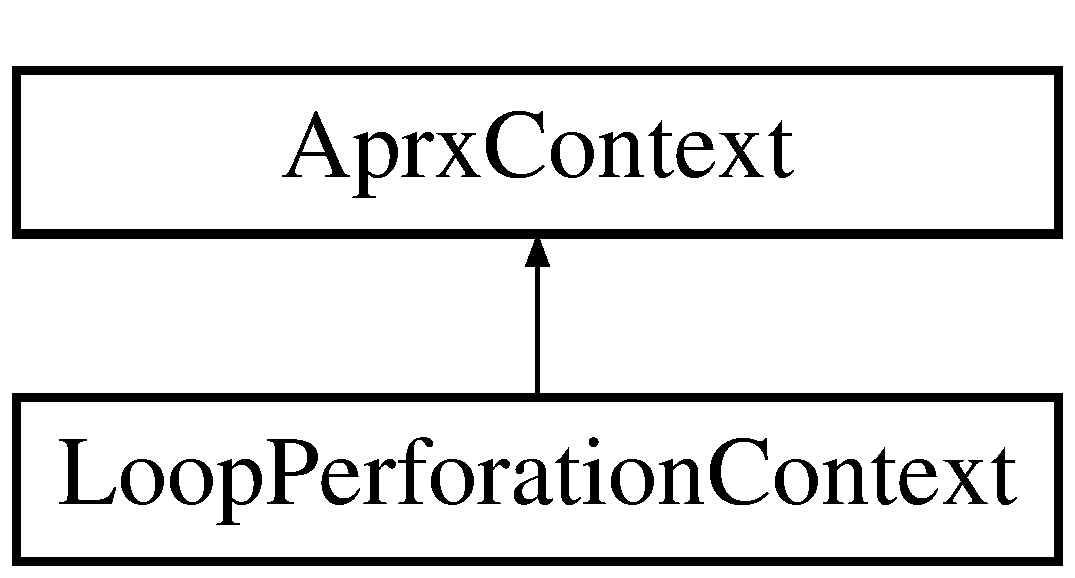
\includegraphics[height=2.000000cm]{classLoopPerforationContext}
\end{center}
\end{figure}
\subsection*{Public Member Functions}
\begin{DoxyCompactItemize}
\item 
\hypertarget{classLoopPerforationContext_a45eb54006f208abc979cfd6d7c776f8b}{}\label{classLoopPerforationContext_a45eb54006f208abc979cfd6d7c776f8b} 
{\bfseries Loop\+Perforation\+Context} (unsigned id, const \+::std\+::string \&desc, const \+::std\+::string \&op\+Id)
\item 
\hypertarget{classLoopPerforationContext_aeb059a73cd5bacdd4041aad1732d72d6}{}\label{classLoopPerforationContext_aeb059a73cd5bacdd4041aad1732d72d6} 
const \+::std\+::string \& {\bfseries get\+Op\+Id} () const
\item 
\hypertarget{classLoopPerforationContext_afea00e355a9afbdcfbc9c9d63ebe1020}{}\label{classLoopPerforationContext_afea00e355a9afbdcfbc9c9d63ebe1020} 
void {\bfseries set\+Op\+Id} (const \+::std\+::string \&op\+Id)
\item 
\hypertarget{classLoopPerforationContext_ad90eeb628f0ddaeafceb7b85c51ce6cb}{}\label{classLoopPerforationContext_ad90eeb628f0ddaeafceb7b85c51ce6cb} 
virtual \+::std\+::vector$<$\+::std\+::string $>$ {\bfseries get\+Global\+Value\+Names} () const override
\item 
\hypertarget{classLoopPerforationContext_a54079a60dd33dd2a66d3f3176898cd39}{}\label{classLoopPerforationContext_a54079a60dd33dd2a66d3f3176898cd39} 
virtual void {\bfseries apply\+Approximation} (\+::iideaa\+::\+Aprx\+Grade, \+::std\+::vector$<$ uint64\+\_\+t $>$) const override
\item 
\hypertarget{classLoopPerforationContext_a4911da63983deebe1a67bd987d1aae66}{}\label{classLoopPerforationContext_a4911da63983deebe1a67bd987d1aae66} 
virtual \+::std\+::vector$<$\+::std\+::string $>$ {\bfseries apply\+Approximation} (\+::iideaa\+::\+Aprx\+Grade g) const override
\item 
\hypertarget{classLoopPerforationContext_a3925e62655b165b134125d0694199742}{}\label{classLoopPerforationContext_a3925e62655b165b134125d0694199742} 
virtual \+::iideaa\+::\+Aprx\+Grade {\bfseries get\+Max\+Applicable\+Grade} () const override
\item 
\hypertarget{classLoopPerforationContext_a97ac37b858e457a35adbea91fd3e9883}{}\label{classLoopPerforationContext_a97ac37b858e457a35adbea91fd3e9883} 
virtual void {\bfseries dump} (\+::llvm\+::raw\+\_\+ostream \&out=\+::llvm\+::outs()) const override
\end{DoxyCompactItemize}


The documentation for this class was generated from the following file\+:\begin{DoxyCompactItemize}
\item 
/home/ntonjeta/sharedfolder/bellerophon/include/\+Plugins/Loop\+Perforation\+Aprx.\+h\end{DoxyCompactItemize}

\hypertarget{classbellerophon_1_1engine_1_1ModuleHelper}{}\section{bellerophon\+:\+:engine\+:\+:Module\+Helper Class Reference}
\label{classbellerophon_1_1engine_1_1ModuleHelper}\index{bellerophon\+::engine\+::\+Module\+Helper@{bellerophon\+::engine\+::\+Module\+Helper}}


The documentation for this class was generated from the following file\+:\begin{DoxyCompactItemize}
\item 
/home/ntonjeta/sharedfolder/bellerophon/include/\+Execution\+Engine\+Helper/Execution\+Engine\+Helper.\+h\end{DoxyCompactItemize}

\chapter{File Documentation}
\hypertarget{Log_8h}{}\section{/home/ntonjeta/sharedfolder/bellerophon/include/\+Log.h File Reference}
\label{Log_8h}\index{/home/ntonjeta/sharedfolder/bellerophon/include/\+Log.\+h@{/home/ntonjeta/sharedfolder/bellerophon/include/\+Log.\+h}}


This file contains a logging facility.  


{\ttfamily \#include \char`\"{}lib/easylogging++.\+h\char`\"{}}\newline
\subsection*{Classes}
\begin{DoxyCompactItemize}
\item 
class \hyperlink{classbellerophon_1_1log_1_1BellerophonLogger}{bellerophon\+::log\+::\+Bellerophon\+Logger}
\begin{DoxyCompactList}\small\item\em Bellero\+Logger Class, provides all functions for the logging. \end{DoxyCompactList}\end{DoxyCompactItemize}
\subsection*{Macros}
\begin{DoxyCompactItemize}
\item 
\hypertarget{Log_8h_a5dca5cbbbd18c88445f7c80133daa9f1}{}\label{Log_8h_a5dca5cbbbd18c88445f7c80133daa9f1} 
\#define \hyperlink{Log_8h_a5dca5cbbbd18c88445f7c80133daa9f1}{E\+L\+P\+P\+\_\+\+N\+O\+\_\+\+D\+E\+F\+A\+U\+L\+T\+\_\+\+L\+O\+G\+\_\+\+F\+I\+LE}
\begin{DoxyCompactList}\small\item\em Disable default logs folder. \end{DoxyCompactList}\item 
\hypertarget{Log_8h_afa94127e7b238437414aded1d422547a}{}\label{Log_8h_afa94127e7b238437414aded1d422547a} 
\#define \hyperlink{Log_8h_afa94127e7b238437414aded1d422547a}{E\+L\+P\+P\+\_\+\+D\+I\+S\+A\+B\+L\+E\+\_\+\+D\+E\+F\+A\+U\+L\+T\+\_\+\+C\+R\+A\+S\+H\+\_\+\+H\+A\+N\+D\+L\+I\+NG}
\begin{DoxyCompactList}\small\item\em Disable crash handling. \end{DoxyCompactList}\end{DoxyCompactItemize}
\subsection*{Typedefs}
\begin{DoxyCompactItemize}
\item 
\hypertarget{Log_8h_a8ae9b2698e0d9f6c63bd82f0eeaf2eba}{}\label{Log_8h_a8ae9b2698e0d9f6c63bd82f0eeaf2eba} 
using {\bfseries bellerophon\+::log\+::\+Verbose\+Level} = el\+::base\+::type\+::\+Verbose\+Level
\end{DoxyCompactItemize}


\subsection{Detailed Description}
This file contains a logging facility. 

\begin{DoxyAuthor}{Author}
Antonio Tammaro 
\end{DoxyAuthor}

\hypertarget{Context_8h}{}\section{/home/ntonjeta/sharedfolder/bellerophon/include/\+Plugins/\+Context.h File Reference}
\label{Context_8h}\index{/home/ntonjeta/sharedfolder/bellerophon/include/\+Plugins/\+Context.\+h@{/home/ntonjeta/sharedfolder/bellerophon/include/\+Plugins/\+Context.\+h}}


This file makes visible Approximate Context.  


{\ttfamily \#include \char`\"{}F\+L\+A\+P/\+Flap\+Aprx\+Context.\+h\char`\"{}}\newline


\subsection{Detailed Description}
This file makes visible Approximate Context. 

\begin{DoxyAuthor}{Author}
Antonio Tammaro 
\end{DoxyAuthor}

\hypertarget{Utils_8h}{}\section{/home/ntonjeta/sharedfolder/bellerophon/include/\+Utils.h File Reference}
\label{Utils_8h}\index{/home/ntonjeta/sharedfolder/bellerophon/include/\+Utils.\+h@{/home/ntonjeta/sharedfolder/bellerophon/include/\+Utils.\+h}}


This file contains a utility functions.  


{\ttfamily \#include \char`\"{}llvm/\+A\+D\+T/\+Twine.\+h\char`\"{}}\newline
{\ttfamily \#include $<$map$>$}\newline
{\ttfamily \#include $<$vector$>$}\newline
{\ttfamily \#include $<$string$>$}\newline
\subsection*{Namespaces}
\begin{DoxyCompactItemize}
\item 
 \hyperlink{namespacebellerophon_1_1fs}{bellerophon\+::fs}
\begin{DoxyCompactList}\small\item\em Filesystem functions. \end{DoxyCompactList}\item 
 \hyperlink{namespacebellerophon_1_1syntax}{bellerophon\+::syntax}
\begin{DoxyCompactList}\small\item\em Syntax checker. \end{DoxyCompactList}\end{DoxyCompactItemize}
\subsection*{Typedefs}
\begin{DoxyCompactItemize}
\item 
using \hyperlink{Utils_8h_a60b7871e9e7675d9765daa9999245bb6}{bellerophon\+::conf\+::\+Fun\+Op\+Conf\+Map} = std\+::map$<$ std\+::string, std\+::vector$<$ std\+::string $>$$>$
\begin{DoxyCompactList}\small\item\em For each function name contains the vector of operator to apply. The Fun\+Op configuration file is a csv file, in which the first element of every row is the name of a function that should be present in the source code, the others comma-\/separated value in the row are the operator\textquotesingle{}s identifier for the correspondent operator to use. \end{DoxyCompactList}\end{DoxyCompactItemize}
\subsection*{Functions}
\begin{DoxyCompactItemize}
\item 
bool \hyperlink{Utils_8h_a404c92d6137c3bda40376e2da18a5bba}{bellerophon\+::conf\+::read\+Functions\+Operators\+Conf\+File} (const std\+::string \&filename, Fun\+Op\+Conf\+Map \&file\+Map)
\begin{DoxyCompactList}\small\item\em Reaf a functions/operators configuration file and create a Fun\+Op\+Conf\+Map. \end{DoxyCompactList}\item 
char \hyperlink{namespacebellerophon_1_1fs_a5fdf1fe521ee409381f36acf1457a858}{bellerophon\+::fs\+::get\+Path\+Separator} ()
\item 
std\+::string \hyperlink{namespacebellerophon_1_1fs_acd4c35b60168bc21d107608e56128664}{bellerophon\+::fs\+::get\+Parent\+Path} (const std\+::string \&)
\begin{DoxyCompactList}\small\item\em Get the parent directory of a path. \end{DoxyCompactList}\item 
bool \hyperlink{namespacebellerophon_1_1fs_a863646cc2d1337eb038f7fdb45012a3a}{bellerophon\+::fs\+::create\+Directories} (const llvm\+::\+Twine \&path, bool ignore\+Existing=true)
\begin{DoxyCompactList}\small\item\em Create directories e sub-\/directories. \end{DoxyCompactList}\item 
\hypertarget{namespacebellerophon_1_1fs_ad2da81a3ede3323f05544977de6d3408}{}\label{namespacebellerophon_1_1fs_ad2da81a3ede3323f05544977de6d3408} 
void {\bfseries bellerophon\+::fs\+::delete\+Directory} (const llvm\+::\+Twine \&path)
\end{DoxyCompactItemize}
\subsection*{Variables}
\begin{DoxyCompactItemize}
\item 
\hypertarget{namespacebellerophon_1_1fs_a058ef4b019d24eea183b04e5da71c288}{}\label{namespacebellerophon_1_1fs_a058ef4b019d24eea183b04e5da71c288} 
const char {\bfseries bellerophon\+::fs\+::path\+Sep}
\end{DoxyCompactItemize}


\subsection{Detailed Description}
This file contains a utility functions. 

\begin{DoxyAuthor}{Author}
Antonio Tammaro 
\end{DoxyAuthor}


\subsection{Typedef Documentation}
\hypertarget{Utils_8h_file_a60b7871e9e7675d9765daa9999245bb6}{}\label{Utils_8h_file_a60b7871e9e7675d9765daa9999245bb6} 
\index{Utils.\+h@{Utils.\+h}!Fun\+Op\+Conf\+Map@{Fun\+Op\+Conf\+Map}}
\index{Fun\+Op\+Conf\+Map@{Fun\+Op\+Conf\+Map}!Utils.\+h@{Utils.\+h}}
\subsubsection{\texorpdfstring{Fun\+Op\+Conf\+Map}{FunOpConfMap}}
{\footnotesize\ttfamily using \hyperlink{Utils_8h_a60b7871e9e7675d9765daa9999245bb6}{bellerophon\+::conf\+::\+Fun\+Op\+Conf\+Map} = typedef std\+::map$<$std\+::string, std\+::vector$<$std\+::string$>$$>$}



For each function name contains the vector of operator to apply. The Fun\+Op configuration file is a csv file, in which the first element of every row is the name of a function that should be present in the source code, the others comma-\/separated value in the row are the operator\textquotesingle{}s identifier for the correspondent operator to use. 

If the first element of the first row is empty, it\textquotesingle{}s possible to specify only the operators that will be applied to all functions found.

To comment a configuration entry use -\/$>$ //. 

\subsection{Function Documentation}
\hypertarget{Utils_8h_file_a404c92d6137c3bda40376e2da18a5bba}{}\label{Utils_8h_file_a404c92d6137c3bda40376e2da18a5bba} 
\index{Utils.\+h@{Utils.\+h}!read\+Functions\+Operators\+Conf\+File@{read\+Functions\+Operators\+Conf\+File}}
\index{read\+Functions\+Operators\+Conf\+File@{read\+Functions\+Operators\+Conf\+File}!Utils.\+h@{Utils.\+h}}
\subsubsection{\texorpdfstring{read\+Functions\+Operators\+Conf\+File()}{readFunctionsOperatorsConfFile()}}
{\footnotesize\ttfamily bool bellerophon\+::conf\+::read\+Functions\+Operators\+Conf\+File (\begin{DoxyParamCaption}\item[{const std\+::string \&}]{filename,  }\item[{\hyperlink{Utils_8h_a60b7871e9e7675d9765daa9999245bb6}{Fun\+Op\+Conf\+Map} \&}]{file\+Map }\end{DoxyParamCaption})}



Reaf a functions/operators configuration file and create a Fun\+Op\+Conf\+Map. 


\begin{DoxyRetVals}{Return values}
{\em bool} & If some error is encountered. \\
\hline
\end{DoxyRetVals}

\hypertarget{Log_8cpp}{}\section{/home/ntonjeta/sharedfolder/bellerophon/src/\+Log.cpp File Reference}
\label{Log_8cpp}\index{/home/ntonjeta/sharedfolder/bellerophon/src/\+Log.\+cpp@{/home/ntonjeta/sharedfolder/bellerophon/src/\+Log.\+cpp}}


This file contains a logging facility.  


{\ttfamily \#include \char`\"{}Log.\+h\char`\"{}}\newline


\subsection{Detailed Description}
This file contains a logging facility. 

\begin{DoxyAuthor}{Author}
Antonio Tammaro 
\end{DoxyAuthor}

\hypertarget{Utils_8cpp}{}\section{/home/ntonjeta/sharedfolder/bellerophon/src/\+Utils.cpp File Reference}
\label{Utils_8cpp}\index{/home/ntonjeta/sharedfolder/bellerophon/src/\+Utils.\+cpp@{/home/ntonjeta/sharedfolder/bellerophon/src/\+Utils.\+cpp}}


This file implements a utility functions.  


{\ttfamily \#include \char`\"{}Utils.\+h\char`\"{}}\newline
{\ttfamily \#include \char`\"{}llvm/\+Support/\+File\+System.\+h\char`\"{}}\newline
{\ttfamily \#include \char`\"{}llvm/\+Support/\+Path.\+h\char`\"{}}\newline
{\ttfamily \#include $<$fstream$>$}\newline
{\ttfamily \#include $<$sstream$>$}\newline
\subsection*{Typedefs}
\begin{DoxyCompactItemize}
\item 
\hypertarget{Utils_8cpp_ac8d53003529fb2d062d614077fe6857c}{}\label{Utils_8cpp_ac8d53003529fb2d062d614077fe6857c} 
using {\bfseries String\+Vector} = std\+::vector$<$ std\+::string $>$
\end{DoxyCompactItemize}


\subsection{Detailed Description}
This file implements a utility functions. 

\begin{DoxyAuthor}{Author}
Antonio Tammaro 
\end{DoxyAuthor}

%--- End generated contents ---

% Index
\backmatter
\newpage
\phantomsection
\clearemptydoublepage
\addcontentsline{toc}{chapter}{Index}
\printindex

\end{document}
